% This is "sig-alternate.tex" V2.1 April 2013
% This file should be compiled with V2.5 of "sig-alternate.cls" May 2012
%
% This example file demonstrates the use of the 'sig-alternate.cls'
% V2.5 LaTeX2e document class file. It is for those submitting
% articles to ACM Conference Proceedings WHO DO NOT WISH TO
% STRICTLY ADHERE TO THE SIGS (PUBS-BOARD-ENDORSED) STYLE.
% The 'sig-alternate.cls' file will produce a similar-looking,
% albeit, 'tighter' paper resulting in, invariably, fewer pages.
%
% ----------------------------------------------------------------------------------------------------------------
% This .tex file (and associated .cls V2.5) produces:
%       1) The Permission Statement
%       2) The Conference (location) Info information
%       3) The Copyright Line with ACM data
%       4) NO page numbers
%
% as against the acm_proc_article-sp.cls file which
% DOES NOT produce 1) thru' 3) above.
%
% Using 'sig-alternate.cls' you have control, however, from within
% the source .tex file, over both the CopyrightYear
% (defaulted to 200X) and the ACM Copyright Data
% (defaulted to X-XXXXX-XX-X/XX/XX).
% e.g.
% \CopyrightYear{2007} will cause 2007 to appear in the copyright line.
% \crdata{0-12345-67-8/90/12} will cause 0-12345-67-8/90/12 to appear in the copyright line.
%
% ---------------------------------------------------------------------------------------------------------------
% This .tex source is an example which *does* use
% the .bib file (from which the .bbl file % is produced).
% REMEMBER HOWEVER: After having produced the .bbl file,
% and prior to final submission, you *NEED* to 'insert'
% your .bbl file into your source .tex file so as to provide
% ONE 'self-contained' source file.
%
% ================= IF YOU HAVE QUESTIONS =======================
% Questions regarding the SIGS styles, SIGS policies and
% procedures, Conferences etc. should be sent to
% Adrienne Griscti (griscti@acm.org)
%
% Technical questions _only_ to
% Gerald Murray (murray@hq.acm.org)
%
% Technical questions related to COCO/BBOB to bbob@lri.fr
% ===============================================================
%
% For tracking purposes - this is V2.0 - May 2012

\documentclass{sig-alternate}
\pdfpagewidth=8.5in
\pdfpageheight=11in
\special{papersize=8.5in,11in}

%%%%%%%%%%%%%%%%%%%%%%%%%%%%%%%%%%%%%%%%%%%%%%%%%%%%%%
% Packages
\usepackage{graphicx}
\usepackage{tabularx}
\usepackage[dvipsnames]{xcolor}
\usepackage{xspace}
\usepackage{float}
\usepackage{rotating}
\usepackage{xstring} % for string operations
\usepackage{wasysym} % Table legend with symbols input from post-processing
\usepackage{MnSymbol} % Table legend with symbols input from post-processing
%\usepackage[hidelinks]{hyperref} % make COCO papers clickable

%%%%%%%%%%%%%%%%%%%%%%%%%%%%%%%%%%%%%%%%%%%%%%%%%%%%%%
% Definitions

% Algorithm names as they appear in the tables, uncomment if necessary
%\newcommand{\algAtables}{\algaperfprof}  % first argument in the post-processing
% \newcommand{\algBtables}{\algbperfprof}  % first argument in the post-processing
% \newcommand{\algCtables}{\algcperfprof}  % first argument in the post-processing
% \newcommand{\algDtables}{\algdperfprof}  % second argument in the post-processing
% ...
% location of pictures files
\newcommand{\bbobdatapath}{ppdata/}
\input{\bbobdatapath bbob_pproc_commands.tex}
\graphicspath{{\bbobdatapath}}



%%%%%%%%%%%%%%%%%%%%%%%%%%%%%%%%%%%%%%%%%%%%%%%%%%%%%%
% pre-defined commands
\newcommand{\DIM}{\ensuremath{\mathrm{DIM}}}
\newcommand{\aRT}{\ensuremath{\mathrm{aRT}}}
\newcommand{\FEvals}{\ensuremath{\mathrm{FEvals}}}
\newcommand{\nruns}{\ensuremath{\mathrm{Nruns}}}
\newcommand{\Df}{\ensuremath{\Delta f}}
\newcommand{\DI}{\ensuremath{\Delta I}}
\newcommand{\nbFEs}{\ensuremath{\mathrm{\#FEs}}}
\newcommand{\fopt}{\ensuremath{f_\mathrm{opt}}}
\newcommand{\ftarget}{\ensuremath{f_\mathrm{t}}}
\newcommand{\Itarget}{\ensuremath{I_\mathrm{target}}}
\newcommand{\CrE}{\ensuremath{\mathrm{CrE}}}
\newcommand{\change}[1]{{\color{red} #1}}
\newcommand{\bbobbiobj}{{\ttfamily bbob-biobj}\xspace}
\newcommand{\hvref}{I^{\mathrm{ref}}}
\newcommand{\TODO}[1]{{\color{red} TODO: #1}}

    \renewcommand{\topfraction}{1}	% max fraction of floats at top
    \renewcommand{\bottomfraction}{1} % max fraction of floats at bottom
    %   Parameters for TEXT pages (not float pages):
    \setcounter{topnumber}{3}
    \setcounter{bottomnumber}{3}
    \setcounter{totalnumber}{3}     % 2 may work better
    \setcounter{dbltopnumber}{4}    % for 2-column pages
    \renewcommand{\dbltopfraction}{1}	% fit big float above 2-col. text
    \renewcommand{\textfraction}{0.0}	% allow minimal text w. figs
    %   Parameters for FLOAT pages (not text pages):
    \renewcommand{\floatpagefraction}{0.80}	% require fuller float pages
    % N.B.: floatpagefraction MUST be less than topfraction !!
    \renewcommand{\dblfloatpagefraction}{0.7}	% require fuller float pages

%%%%%%%%%%%%%%%%%%%%%%%%%%%%%%%%%%%%%%%%%%%%%%%%%%%%%%

\begin{document}

\IfFileExists{\bbobdatapath ppfig2_f001.pdf}{2 algorithms currently not supported}{}

%
% --- Author Metadata here ---
\conferenceinfo{GECCO'17,} {July 1-2, 2017, Berlin, Germany.}
\CopyrightYear{2017}
\crdata{TBA}
\clubpenalty=10000
\widowpenalty = 10000
% --- End of Author Metadata ---

\title{Black-Box Optimization Benchmarking Template for the Comparison of Multiple Algorithms on the Biobjective {\Large \bbobbiobj} Testbed}
\subtitle{Draft version
\titlenote{Submission deadline: March 28th.}}
%Camera-ready paper due April 16th.}}

%
% You need the command \numberofauthors to handle the 'placement
% and alignment' of the authors beneath the title.
%
% For aesthetic reasons, we recommend 'three authors at a time'
% i.e. three 'name/affiliation blocks' be placed beneath the title.
%
% NOTE: You are NOT restricted in how many 'rows' of
% "name/affiliations" may appear. We just ask that you restrict
% the number of 'columns' to three.
%
% Because of the available 'opening page real-estate'
% we ask you to refrain from putting more than six authors
% (two rows with three columns) beneath the article title.
% More than six makes the first-page appear very cluttered indeed.
%
% Use the \alignauthor commands to handle the names
% and affiliations for an 'aesthetic maximum' of six authors.
% Add names, affiliations, addresses for
% the seventh etc. author(s) as the argument for the
% \additionalauthors command.
% These 'additional authors' will be output/set for you
% without further effort on your part as the last section in
% the body of your article BEFORE References or any Appendices.

\numberofauthors{1} %  in this sample file, there are a *total*
% of EIGHT authors. SIX appear on the 'first-page' (for formatting
% reasons) and the remaining two appear in the \additionalauthors section.
%
\author{
% You can go ahead and credit any number of authors here,
% e.g. one 'row of three' or two rows (consisting of one row of three
% and a second row of one, two or three).
%
% The command \alignauthor (no curly braces needed) should
% precede each author name, affiliation/snail-mail address and
% e-mail address. Additionally, tag each line of
% affiliation/address with \affaddr, and tag the
% e-mail address with \email.
%
% 1st. author
\alignauthor
Forename Name\\ %\titlenote{Dr.~Trovato insisted his name be first.}\\
%       \affaddr{Institute for Clarity in Documentation}\\
%       \affaddr{1932 Wallamaloo Lane}\\
%       \affaddr{Wallamaloo, New Zealand}\\
%       \email{trovato@corporation.com}
%% 2nd. author
%\alignauthor
%G.K.M. Tobin\titlenote{The secretary disavows
%any knowledge of this author's actions.}\\
%       \affaddr{Institute for Clarity in Documentation}\\
%       \affaddr{P.O. Box 1212}\\
%       \affaddr{Dublin, Ohio 43017-6221}\\
%       \email{webmaster@marysville-ohio.com}
%% 3rd. author
%\alignauthor Lars Th{\o}rv{\"a}ld\titlenote{This author is the
%one who did all the really hard work.}\\
%       \affaddr{The Th{\o}rv{\"a}ld Group}\\
%       \affaddr{1 Th{\o}rv{\"a}ld Circle}\\
%       \affaddr{Hekla, Iceland}\\
%       \email{larst@affiliation.org}
%\and  % use '\and' if you need 'another row' of author names
%% 4th. author
%\alignauthor Lawrence P. Leipuner\\
%       \affaddr{Brookhaven Laboratories}\\
%       \affaddr{Brookhaven National Lab}\\
%       \affaddr{P.O. Box 5000}\\
%       \email{lleipuner@researchlabs.org}
%% 5th. author
%\alignauthor Sean Fogarty\\
%       \affaddr{NASA Ames Research Center}\\
%       \affaddr{Moffett Field}\\
%       \affaddr{California 94035}\\
%       \email{fogartys@amesres.org}
%% 6th. author
%\alignauthor Charles Palmer\\
%       \affaddr{Palmer Research Laboratories}\\
%       \affaddr{8600 Datapoint Drive}\\
%       \affaddr{San Antonio, Texas 78229}\\
%       \email{cpalmer@prl.com}
} % author
%% There's nothing stopping you putting the seventh, eighth, etc.
%% author on the opening page (as the 'third row') but we ask,
%% for aesthetic reasons that you place these 'additional authors'
%% in the \additional authors block, viz.
%\additionalauthors{Additional authors: John Smith (The Th{\o}rv{\"a}ld Group,
%email: {\texttt{jsmith@affiliation.org}}) and Julius P.~Kumquat
%(The Kumquat Consortium, email: {\texttt{jpkumquat@consortium.net}}).}
%\date{30 July 1999}
%% Just remember to make sure that the TOTAL number of authors
%% is the number that will appear on the first page PLUS the
%% number that will appear in the \additionalauthors section.

\maketitle
\begin{abstract}
to be written
\end{abstract}

% Add any ACM category that you feel is needed, not mandatory anymore
%\category{G.1.6}{Numerical Analysis}{Optimization}[global optimization,
%unconstrained optimization]
%\category{F.2.1}{Analysis of Algorithms and Problem Complexity}{Numerical Algorithms and Problems}

% Complete with anything that is needed
\terms{Algorithms}

% Complete with anything that is needed
\keywords{Benchmarking, Black-box optimization, Bi-objective optimization}

% \section{Introduction}
%
% \section{Algorithm Presentation}
%
% \section{Experimental Procedure}
%

%%%%%%%%%%%%%%%%%%%%%%%%%%%%%%%%%%%%%%%%%%%%%%%%%%%%%%%%%%%%%%%%%%%%%%%%%%%%%%%
\section{CPU Timing}
%%%%%%%%%%%%%%%%%%%%%%%%%%%%%%%%%%%%%%%%%%%%%%%%%%%%%%%%%%%%%%%%%%%%%%%%%%%%%%%
% note that the following text is just a proposal and can/should be changed to your needs:
In order to evaluate the CPU timing of the algorithm, we have run the \change{\algorithmA} with restarts on the entire bbob-biobj test suite \cite{biobj2016func} for $2 D$ function evaluations. The \change{C/Java/Matlab/Octave/Python} code was run on a \change{Mac Intel(R) Core(TM) i5-2400S CPU @ 2.50GHz} with \change{1} processor and \change{4} cores. The time per function evaluation for dimensions 2, 3, 5, 10, 20\change{, 40} equals \change{$x.x$}, \change{$x.x$}, \change{$x.x$}, \change{$xx$}, \change{$xxx$}\change{, and $xxx$} seconds respectively. 

\change{repeat the above for any algorithm tested}

%%%%%%%%%%%%%%%%%%%%%%%%%%%%%%%%%%%%%%%%%%%%%%%%%%%%%%%%%%%%%%%%%%%%%%%%%%%%%%%
\section{Results}
%%%%%%%%%%%%%%%%%%%%%%%%%%%%%%%%%%%%%%%%%%%%%%%%%%%%%%%%%%%%%%%%%%%%%%%%%%%%%%%

Results from experiments according to \cite{hansen2016exp},
\cite{hansen2016perfass} and \cite{biobj2016perfass} on the benchmark
functions given in \cite{biobj2016func} are presented in
Figures~\ref{fig:ECDFsingleOne}, \ref{fig:ECDFsingleTwo}, \ref{fig:ECDFsGroupsFive} and
\ref{fig:ECDFsGroupsTwenty} and in Tables~\ref{tab:aRTs5} and~\ref{tab:aRTs20}.
The experiments were performed with COCO \cite{hansen2016cocoplat}, version
\change{1.0.1}, the plots were produced with version \change{1.1.1}.

The \textbf{average runtime (aRT)}, used in the %figures and
tables,
depends on a given quality indicator value, $\Itarget=\hvref+\DI$, and is
computed over all relevant trials as the number of function
evaluations executed during each trial while the best indicator value
did not reach \Itarget, summed over all trials and divided by the
number of trials that actually reached \Itarget\
\cite{hansen2016exp,price1997dev}.  \textbf{Statistical significance}
is tested with the rank-sum test for a given target $\Itarget$
using, for each trial,
either the number of needed function evaluations to reach
$\Itarget$ (inverted and multiplied by $-1$), or, if the target
was not reached, the best $\DI$-value achieved, measured only up to
the smallest number of overall function evaluations for any
unsuccessful trial under consideration.



%%%%%%%%%%%%%%%%%%%%%%%%%%%%%%%%%%%%%%%%%%%%%%%%%%%%%%%%%%%%%%%%%%%%%%%%%%%%%%%
%%%%%%%%%%%%%%%%%%%%%%%%%%%%%%%%%%%%%%%%%%%%%%%%%%%%%%%%%%%%%%%%%%%%%%%%%%%%%%%

% ECDFs per function in dimension 10

%%%%%%%%%%%%%%%%%%%%%%%%%%%%%%%%%%%%%%%%%%%%%%%%%%%%%%%%%%%%%%%%%%%%%%%%%%%%%%%
\begin{figure*}
\centering
\begin{tabular}{@{\hspace*{-0.005\textwidth}}l@{\hspace*{-0.005\textwidth}}l@{\hspace*{-0.005\textwidth}}l@{\hspace*{-0.005\textwidth}}l@{\hspace*{-0.005\textwidth}}l@{\hspace*{-0.005\textwidth}}}
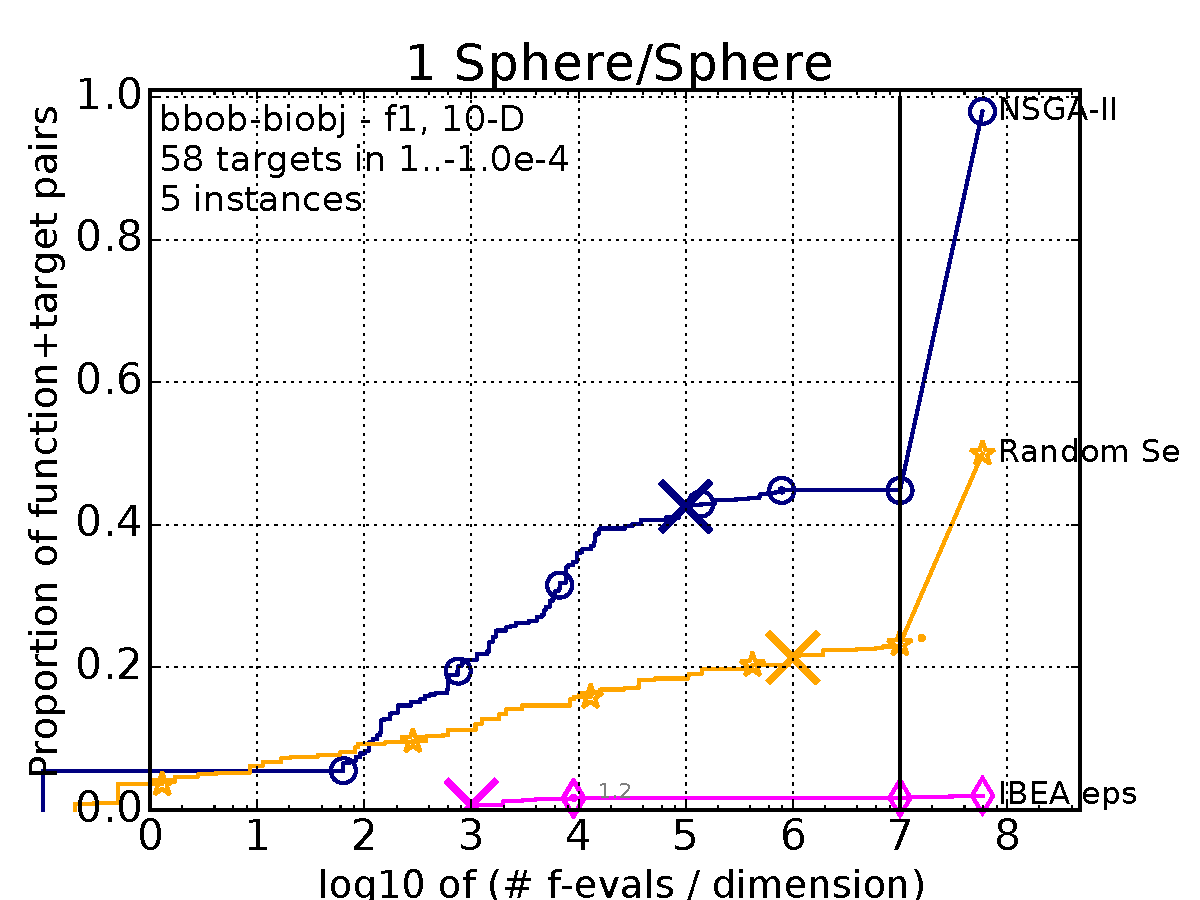
\includegraphics[width=0.2\textwidth]{pprldmany-single-functions/pprldmany_f001_10D}&
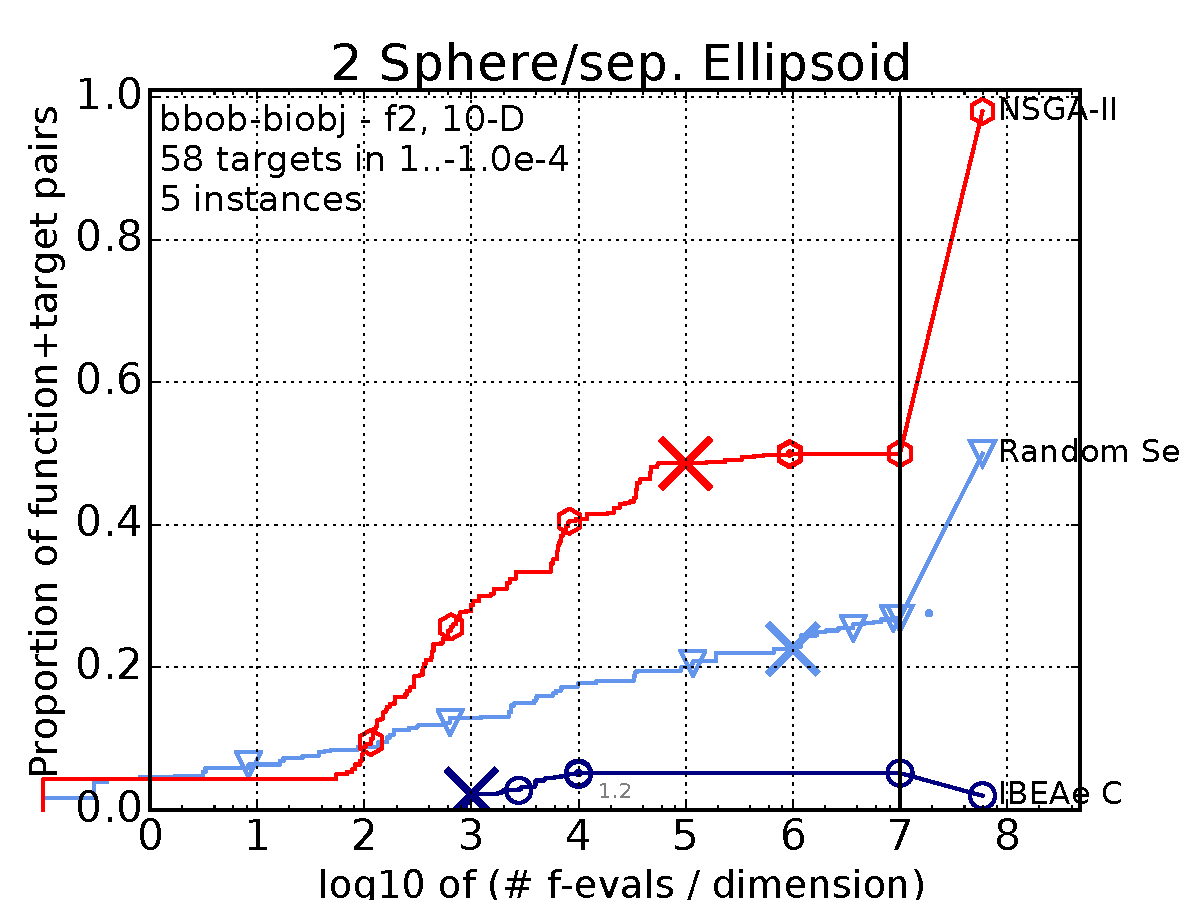
\includegraphics[width=0.2\textwidth]{pprldmany-single-functions/pprldmany_f002_10D}&
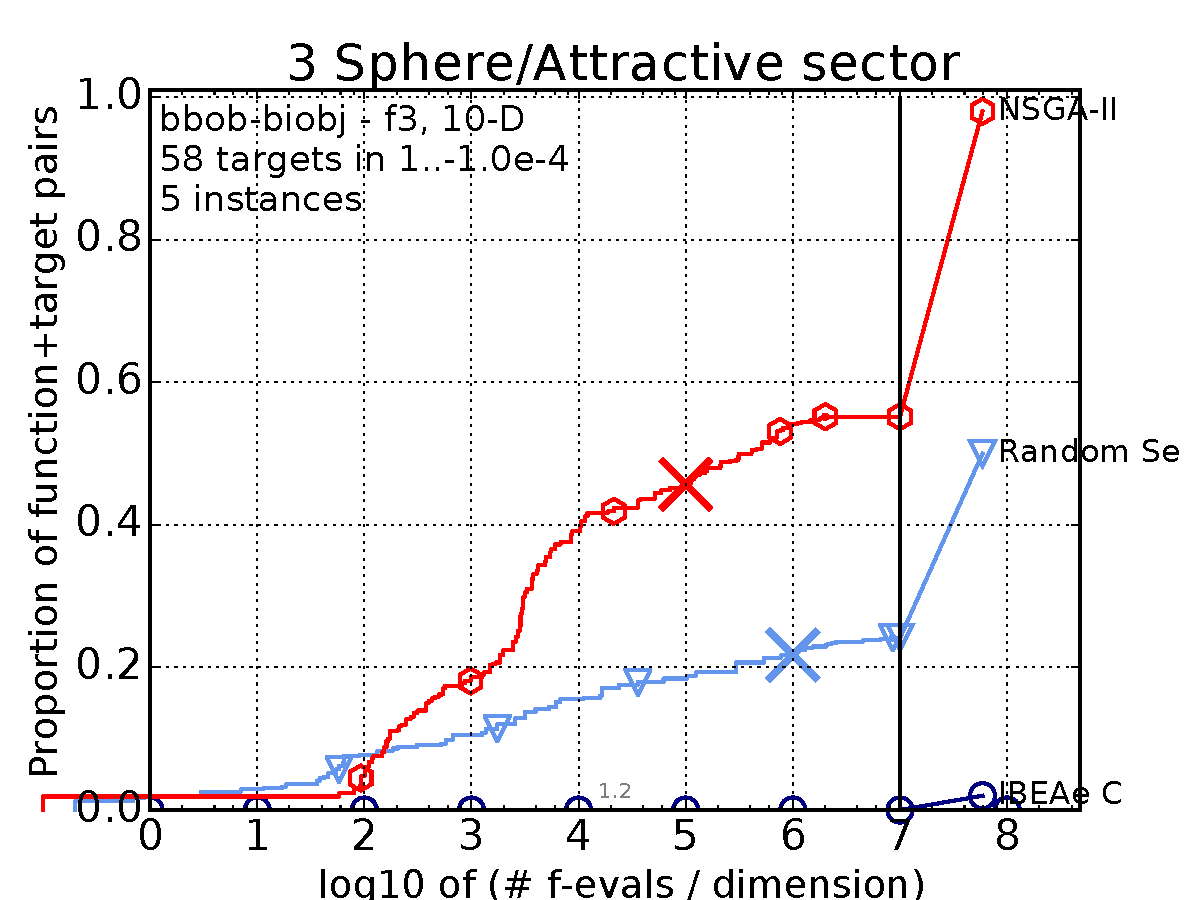
\includegraphics[width=0.2\textwidth]{pprldmany-single-functions/pprldmany_f003_10D}&
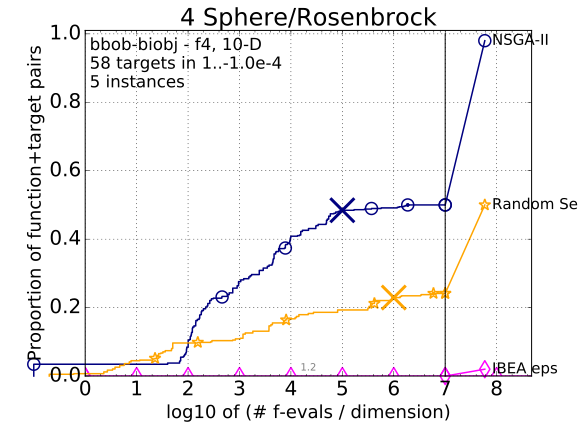
\includegraphics[width=0.2\textwidth]{pprldmany-single-functions/pprldmany_f004_10D}&
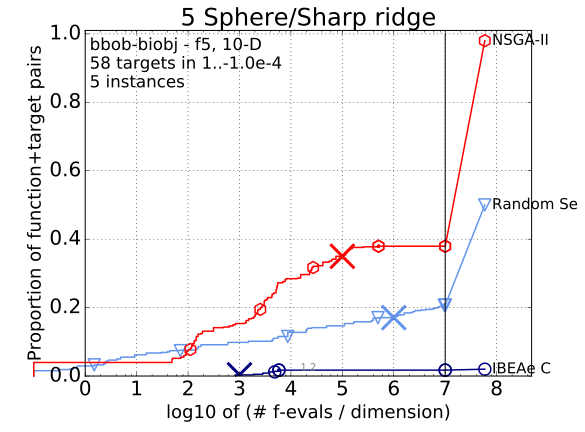
\includegraphics[width=0.2\textwidth]{pprldmany-single-functions/pprldmany_f005_10D}\\[-1.8ex]
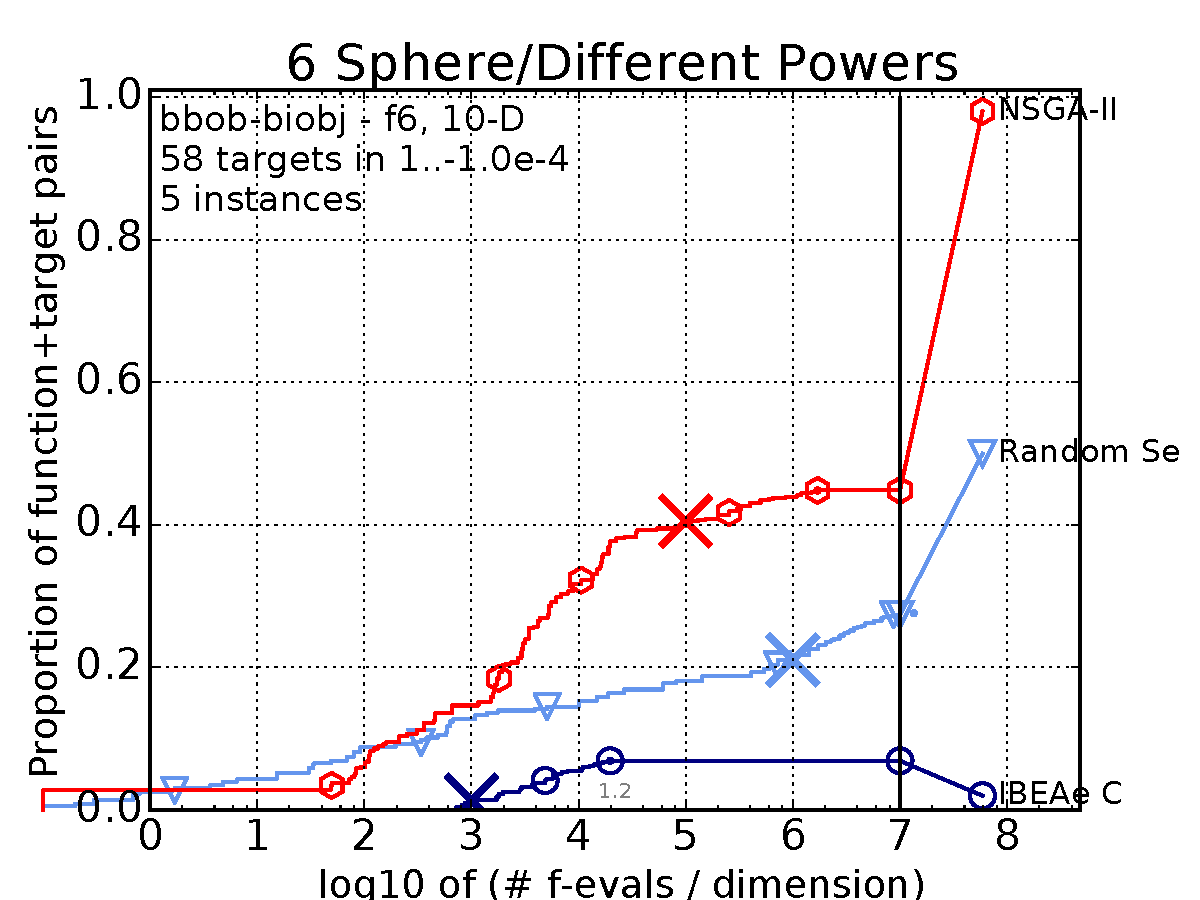
\includegraphics[width=0.2\textwidth]{pprldmany-single-functions/pprldmany_f006_10D}&
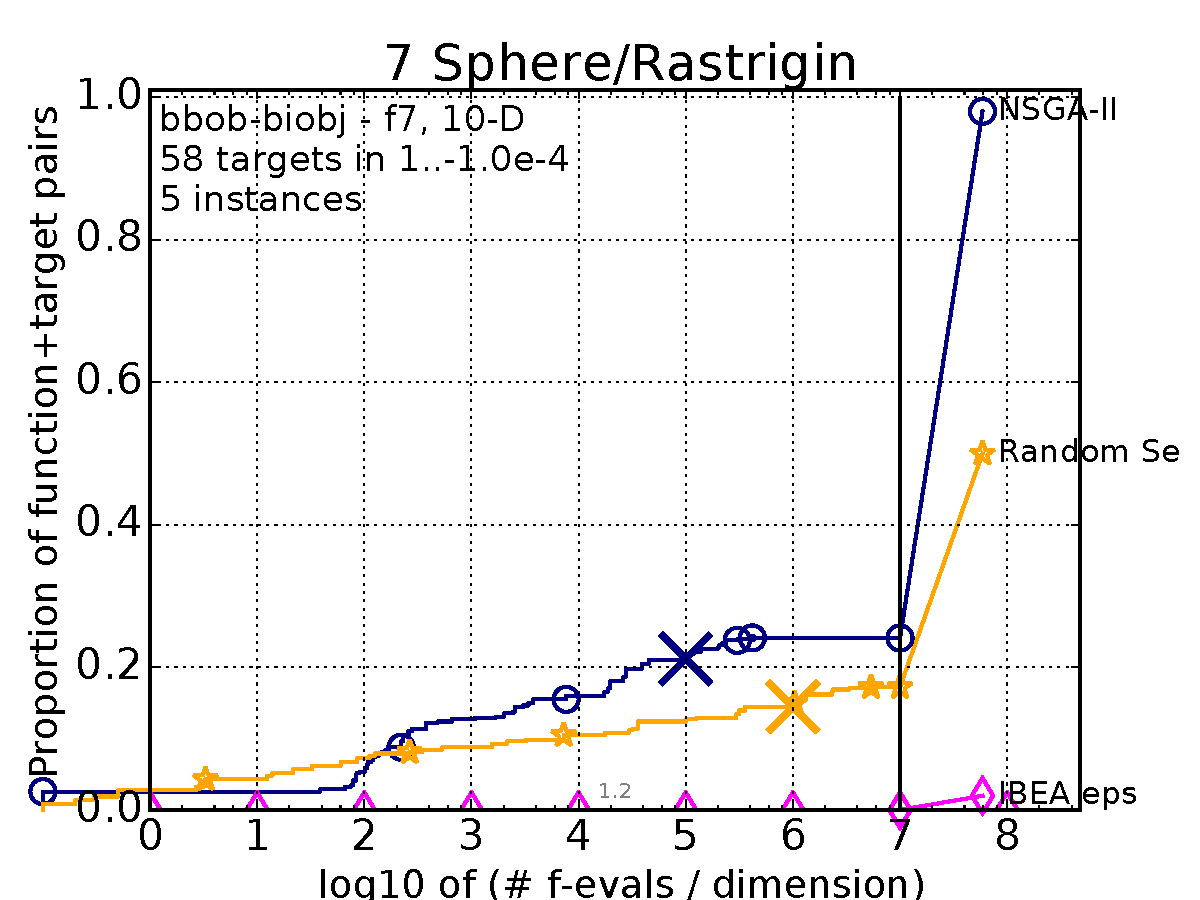
\includegraphics[width=0.2\textwidth]{pprldmany-single-functions/pprldmany_f007_10D}&
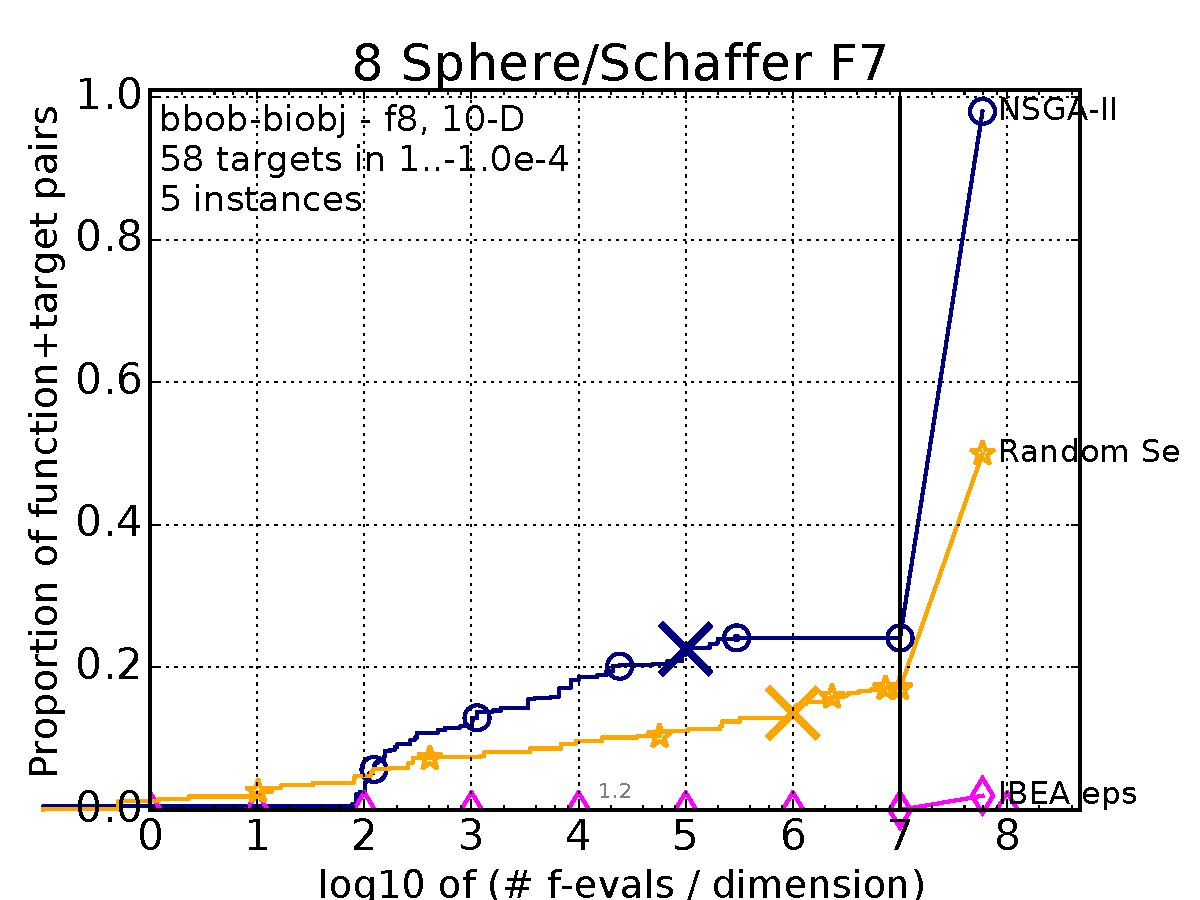
\includegraphics[width=0.2\textwidth]{pprldmany-single-functions/pprldmany_f008_10D}&
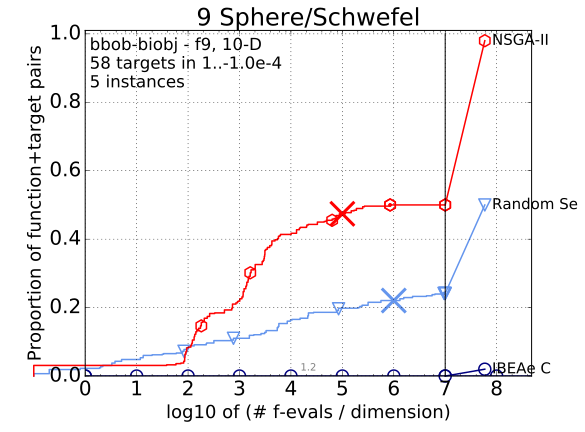
\includegraphics[width=0.2\textwidth]{pprldmany-single-functions/pprldmany_f009_10D}&
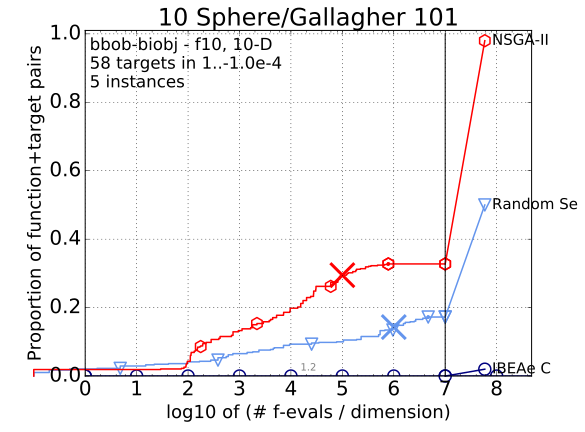
\includegraphics[width=0.2\textwidth]{pprldmany-single-functions/pprldmany_f010_10D}\\[-1.8ex]
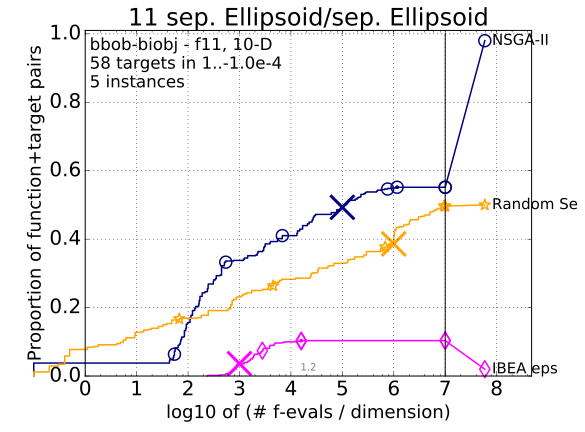
\includegraphics[width=0.2\textwidth]{pprldmany-single-functions/pprldmany_f011_10D}&
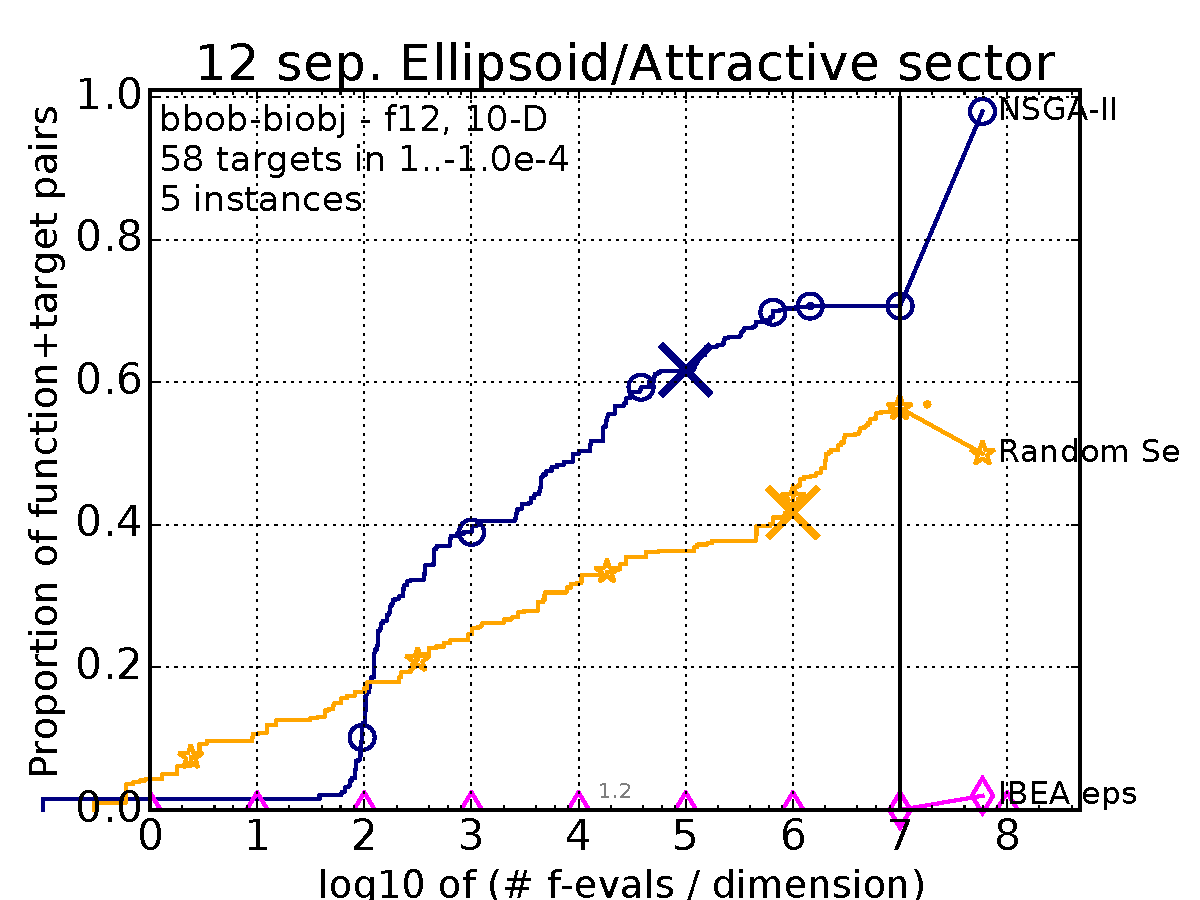
\includegraphics[width=0.2\textwidth]{pprldmany-single-functions/pprldmany_f012_10D}&
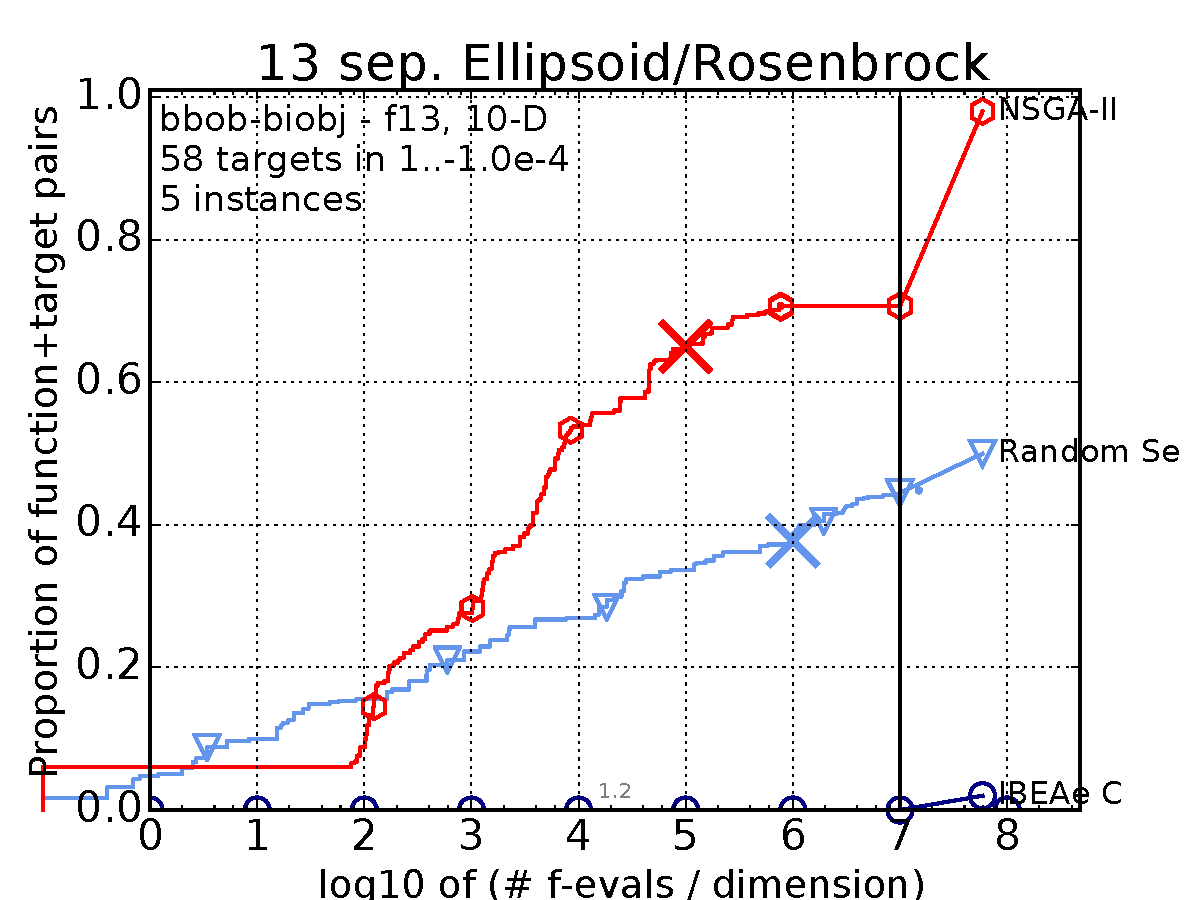
\includegraphics[width=0.2\textwidth]{pprldmany-single-functions/pprldmany_f013_10D}&
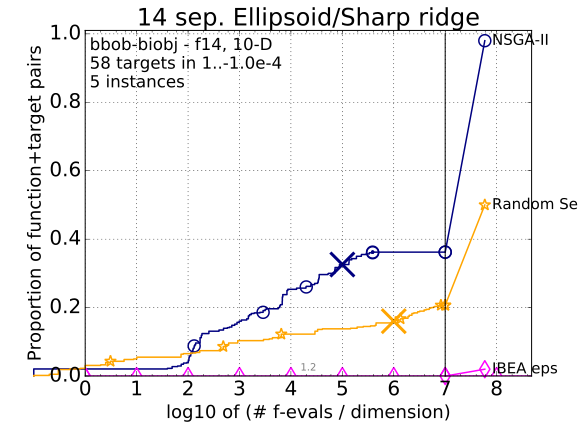
\includegraphics[width=0.2\textwidth]{pprldmany-single-functions/pprldmany_f014_10D}&
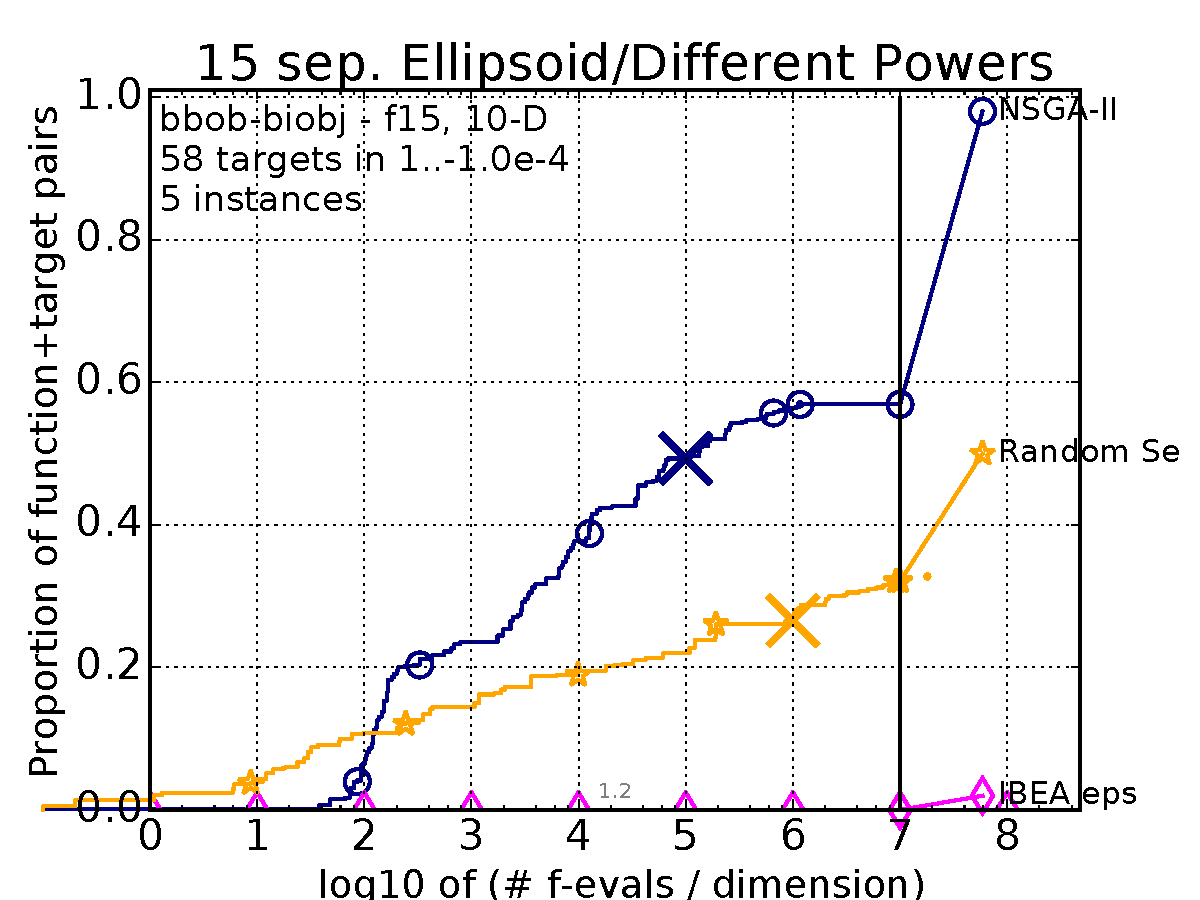
\includegraphics[width=0.2\textwidth]{pprldmany-single-functions/pprldmany_f015_10D}\\[-1.8ex]
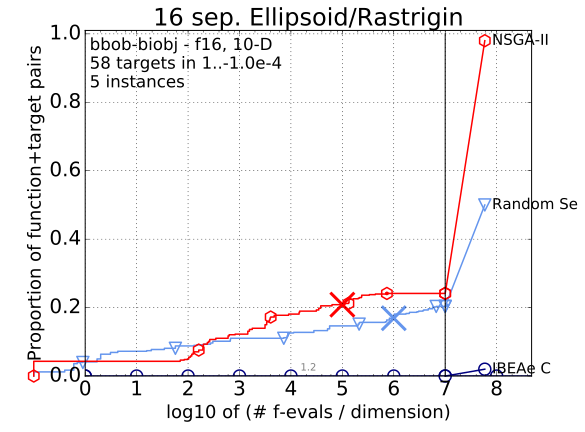
\includegraphics[width=0.2\textwidth]{pprldmany-single-functions/pprldmany_f016_10D}&
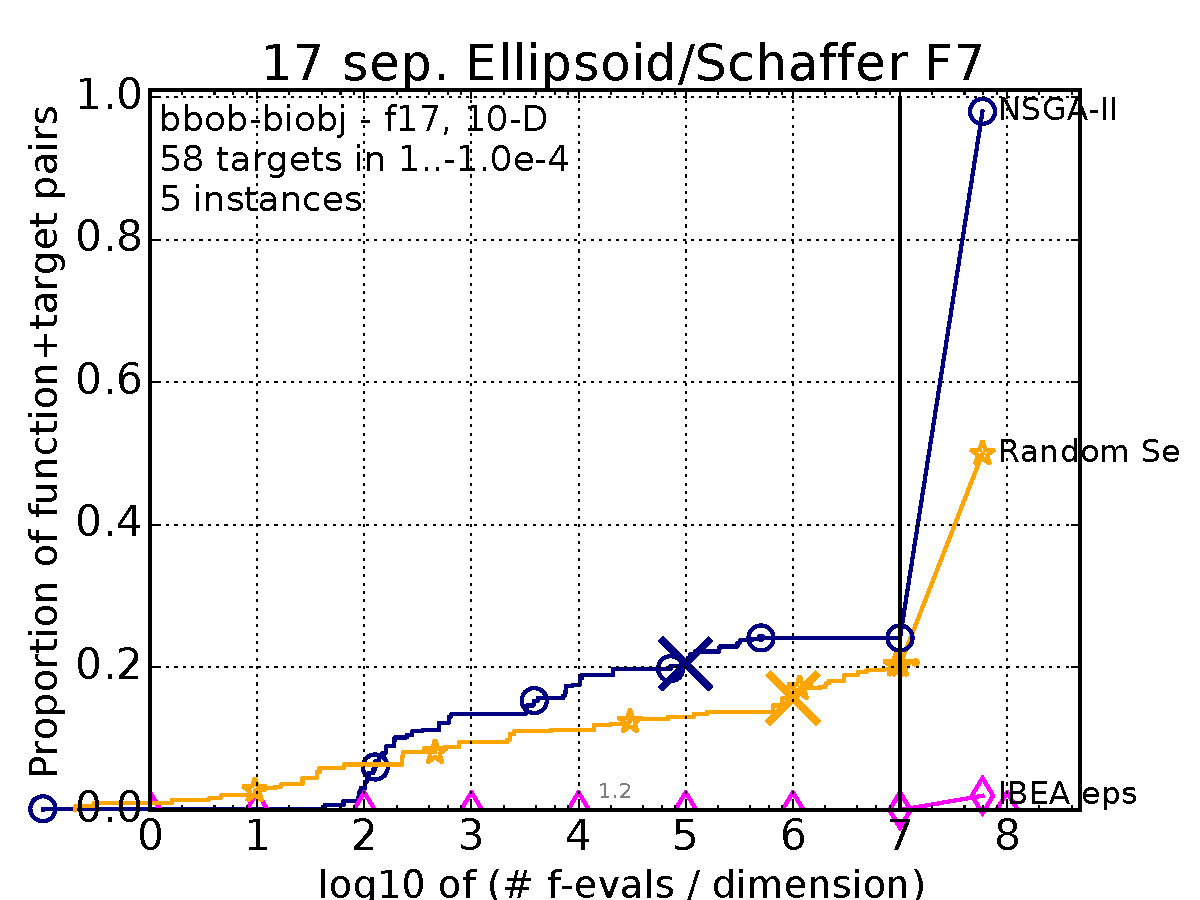
\includegraphics[width=0.2\textwidth]{pprldmany-single-functions/pprldmany_f017_10D}&
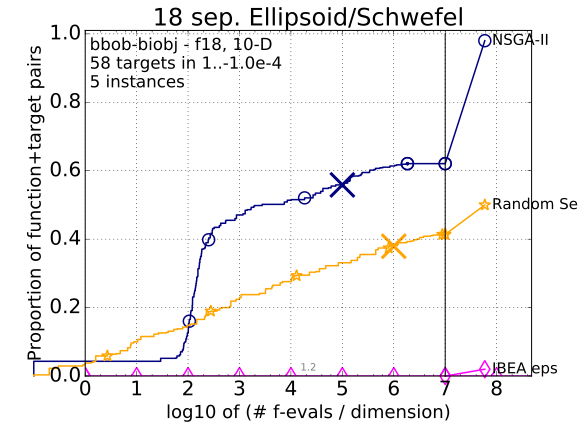
\includegraphics[width=0.2\textwidth]{pprldmany-single-functions/pprldmany_f018_10D}&
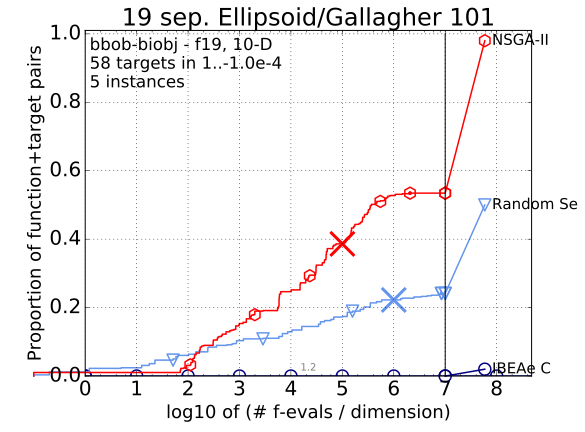
\includegraphics[width=0.2\textwidth]{pprldmany-single-functions/pprldmany_f019_10D}&
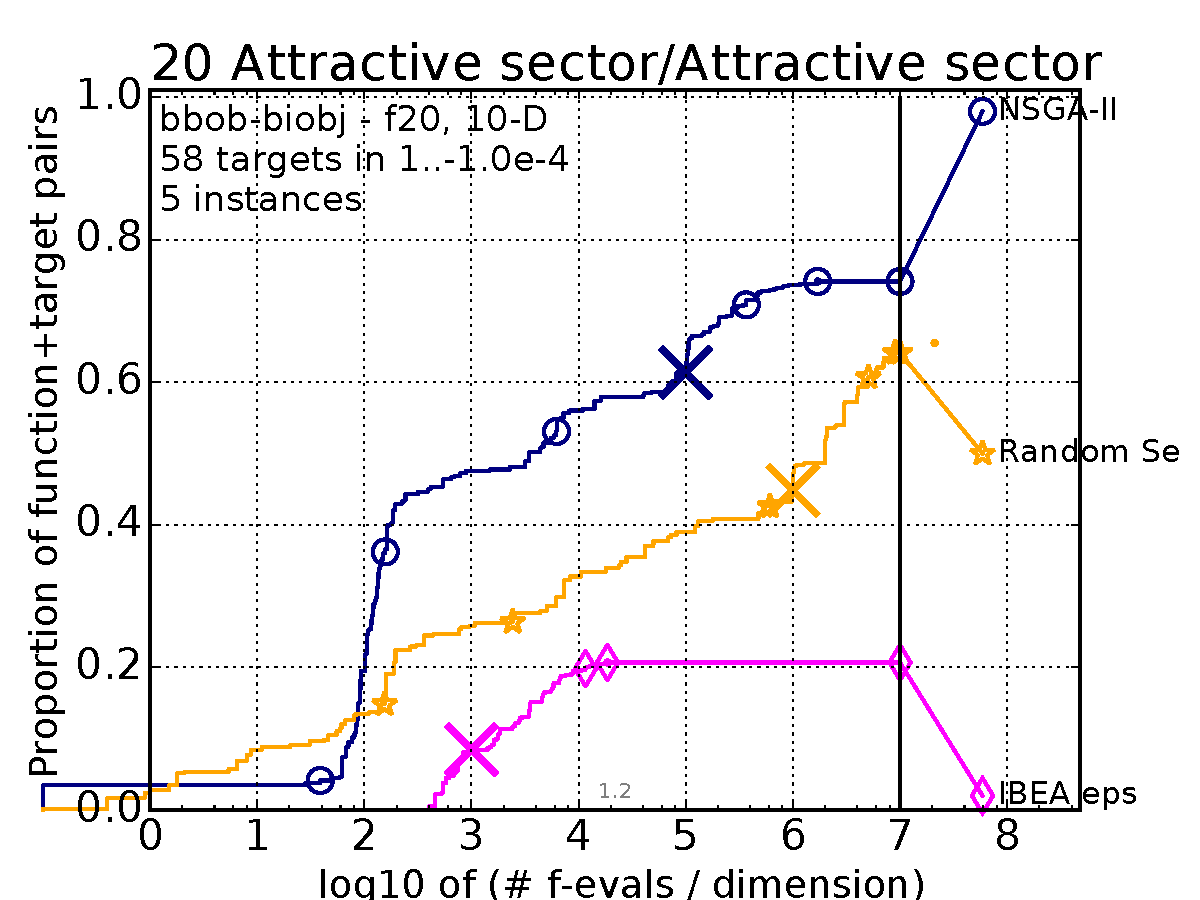
\includegraphics[width=0.2\textwidth]{pprldmany-single-functions/pprldmany_f020_10D}\\[-1.8ex]
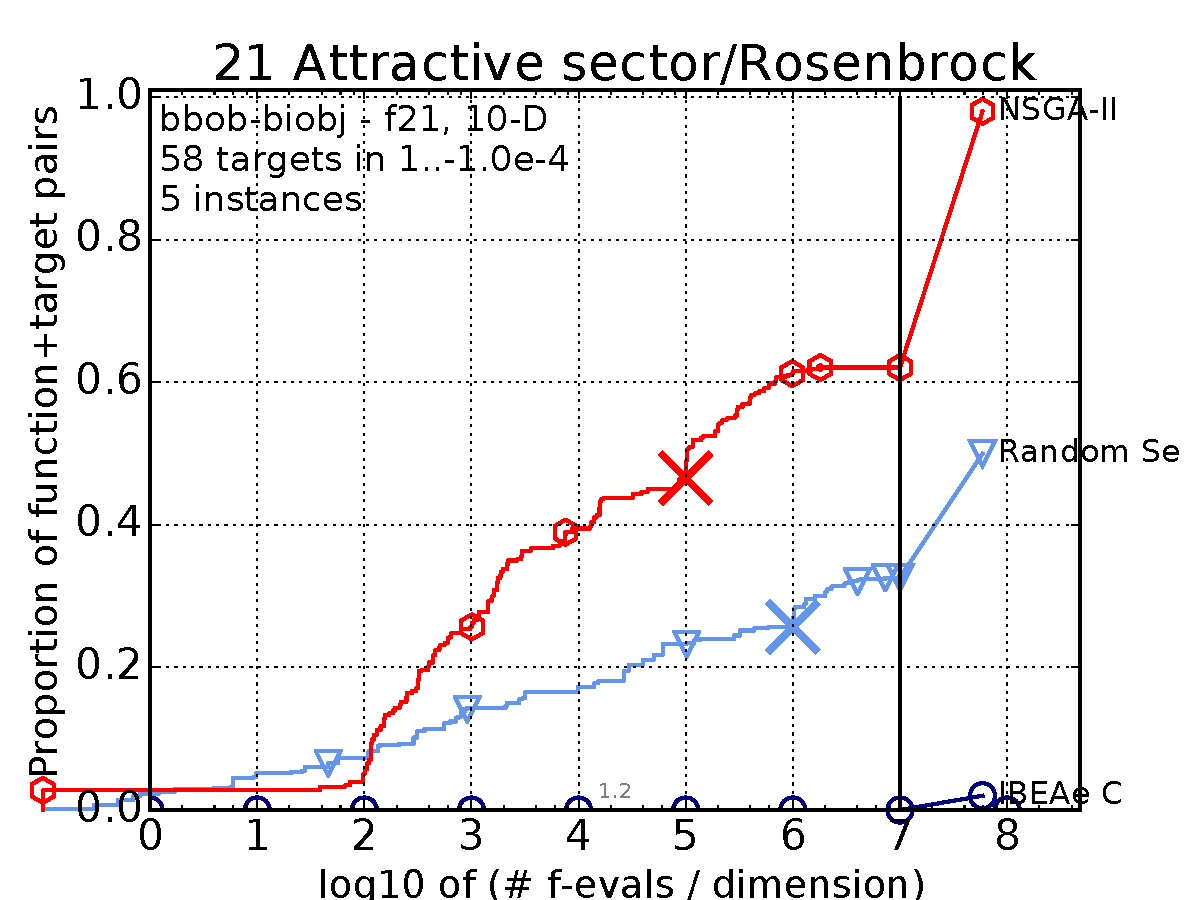
\includegraphics[width=0.2\textwidth]{pprldmany-single-functions/pprldmany_f021_10D}&
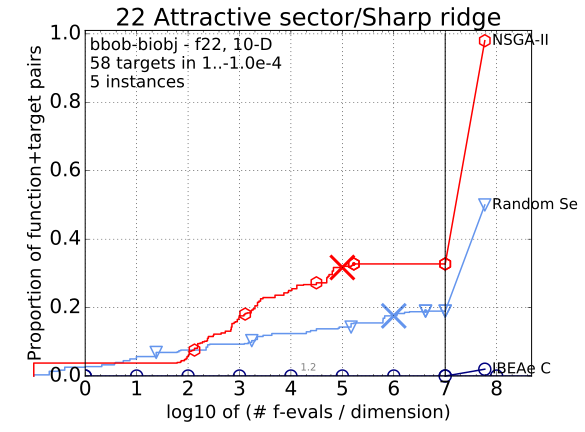
\includegraphics[width=0.2\textwidth]{pprldmany-single-functions/pprldmany_f022_10D}&
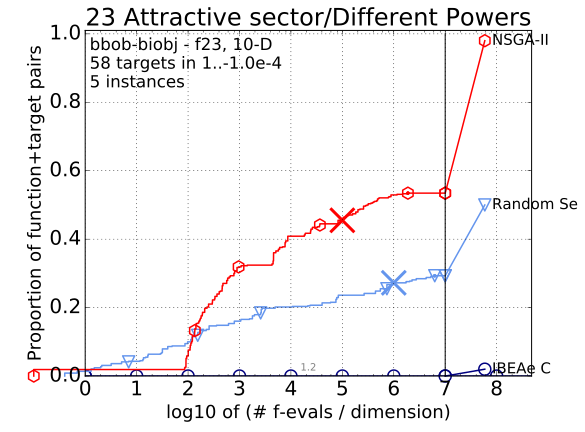
\includegraphics[width=0.2\textwidth]{pprldmany-single-functions/pprldmany_f023_10D}&
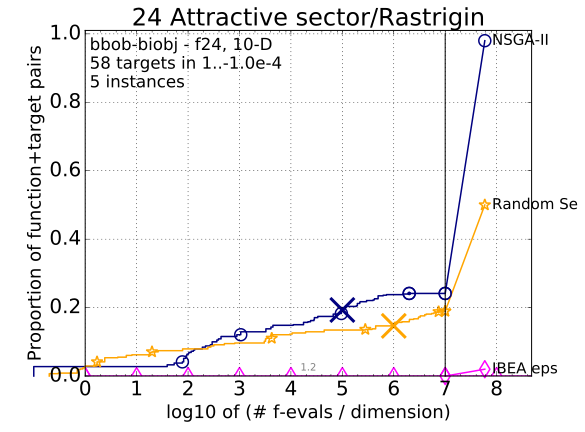
\includegraphics[width=0.2\textwidth]{pprldmany-single-functions/pprldmany_f024_10D}&
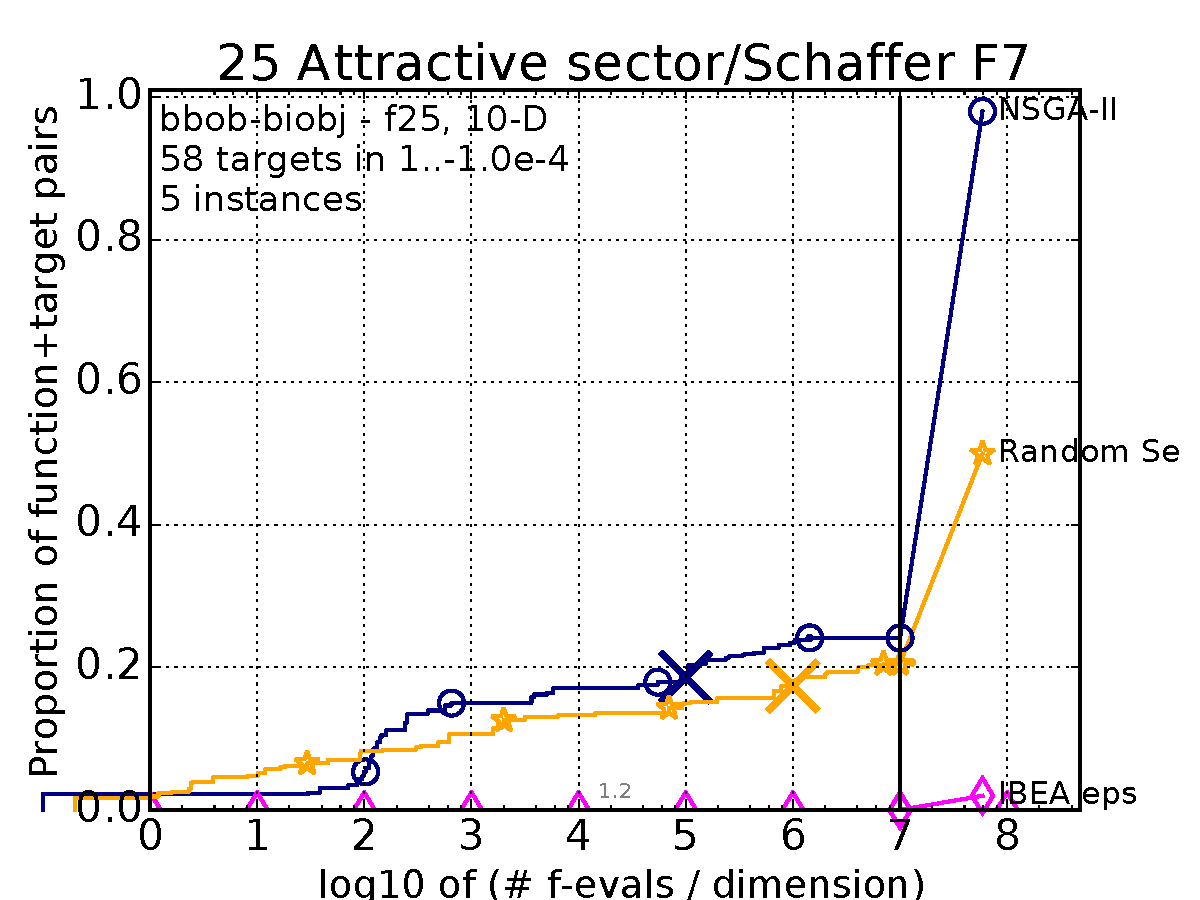
\includegraphics[width=0.2\textwidth]{pprldmany-single-functions/pprldmany_f025_10D}\\[-1.8ex]
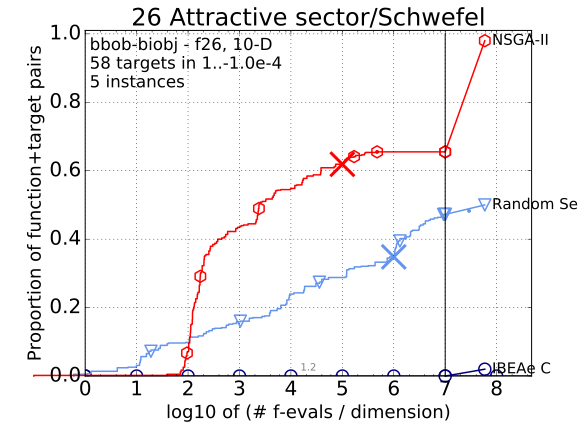
\includegraphics[width=0.2\textwidth]{pprldmany-single-functions/pprldmany_f026_10D}&
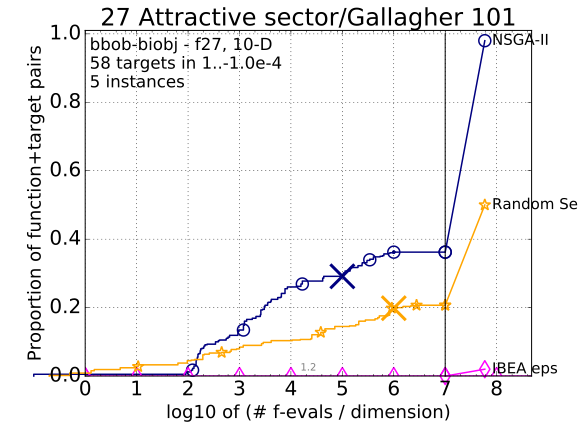
\includegraphics[width=0.2\textwidth]{pprldmany-single-functions/pprldmany_f027_10D}&
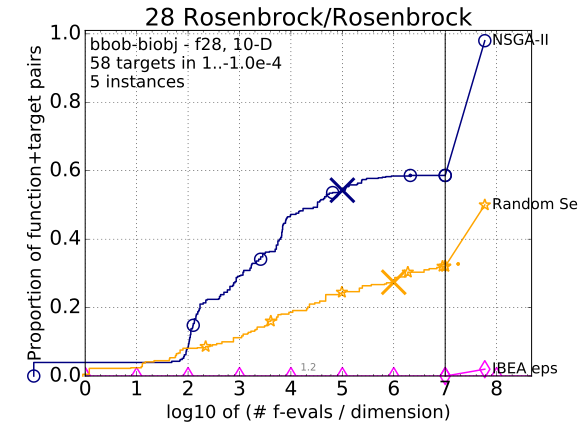
\includegraphics[width=0.2\textwidth]{pprldmany-single-functions/pprldmany_f028_10D}&
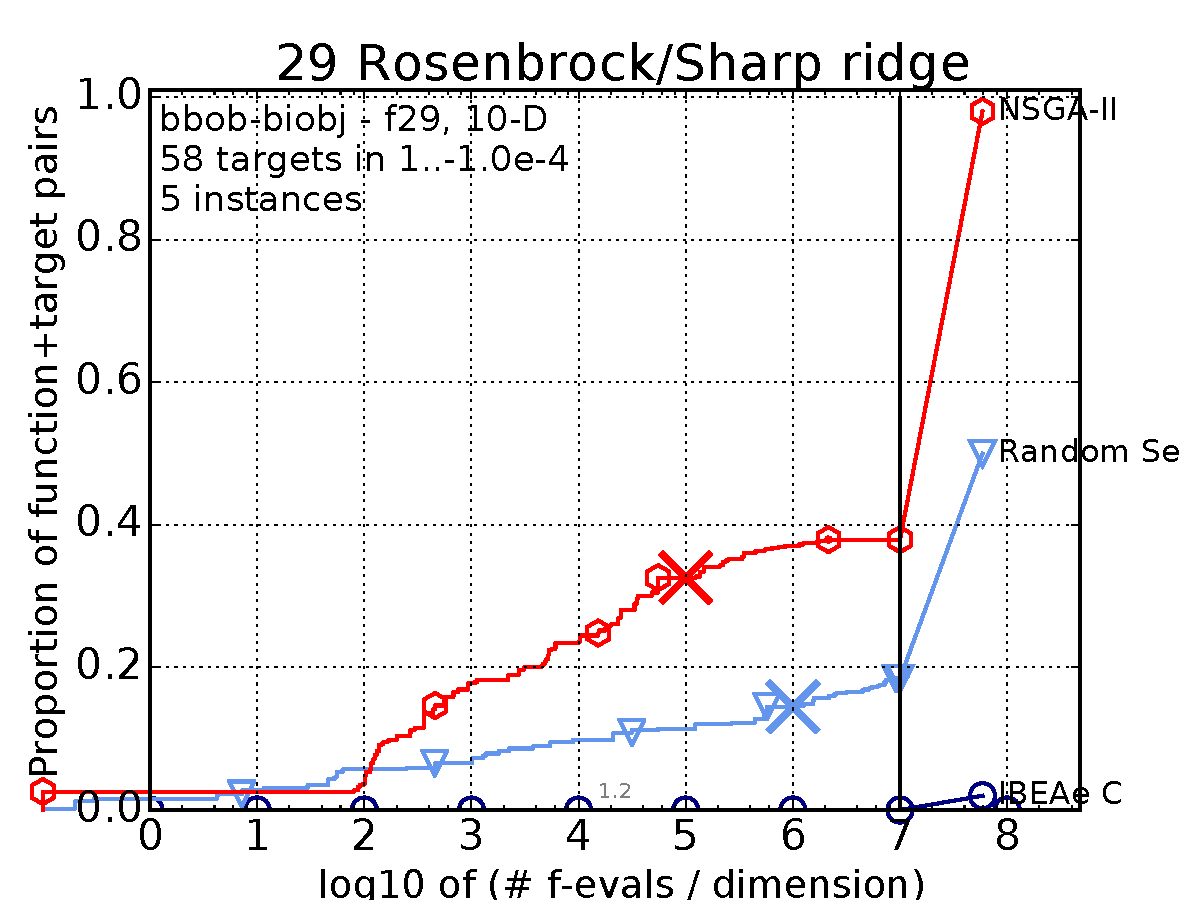
\includegraphics[width=0.2\textwidth]{pprldmany-single-functions/pprldmany_f029_10D}&
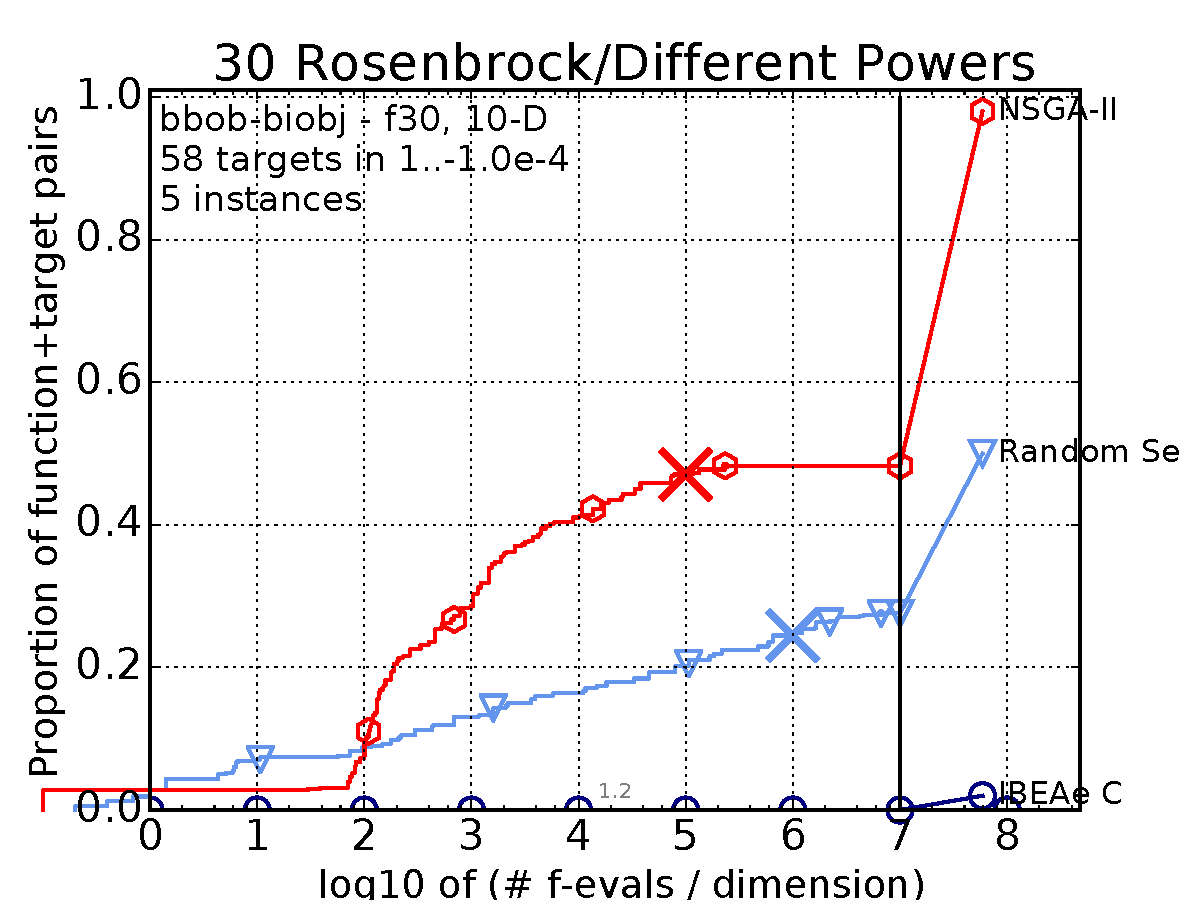
\includegraphics[width=0.2\textwidth]{pprldmany-single-functions/pprldmany_f030_10D}\\[-1.8ex]
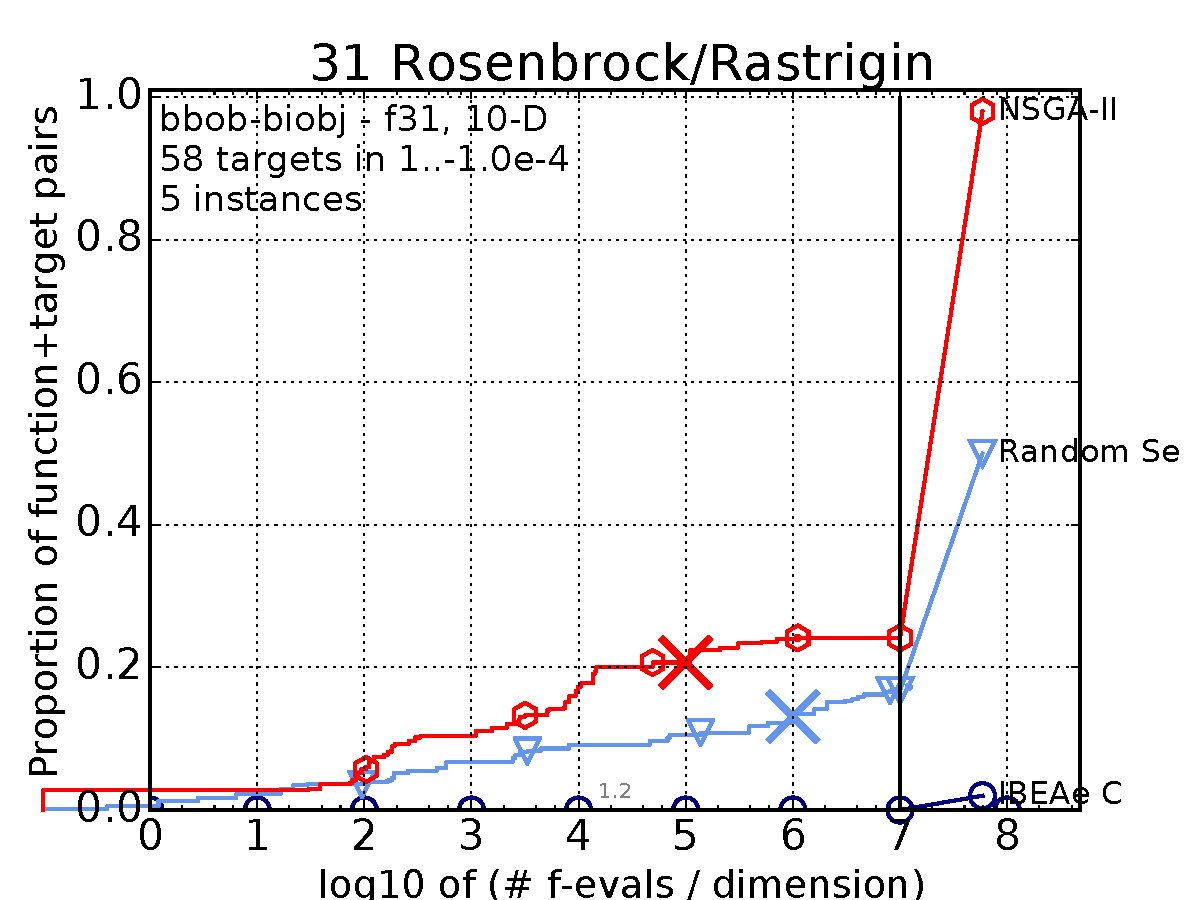
\includegraphics[width=0.2\textwidth]{pprldmany-single-functions/pprldmany_f031_10D}&
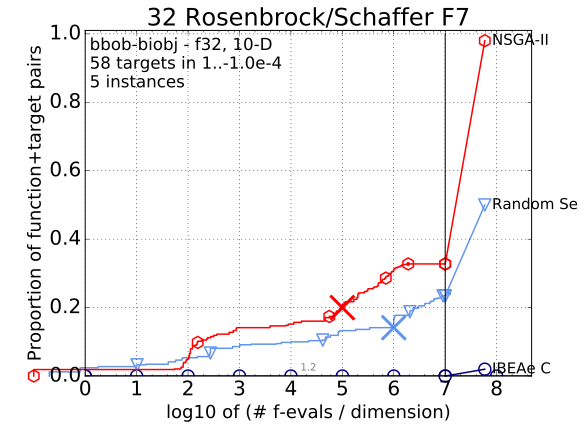
\includegraphics[width=0.2\textwidth]{pprldmany-single-functions/pprldmany_f032_10D}&
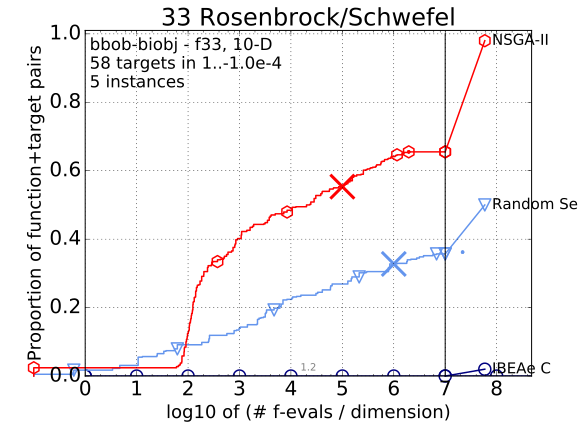
\includegraphics[width=0.2\textwidth]{pprldmany-single-functions/pprldmany_f033_10D}&
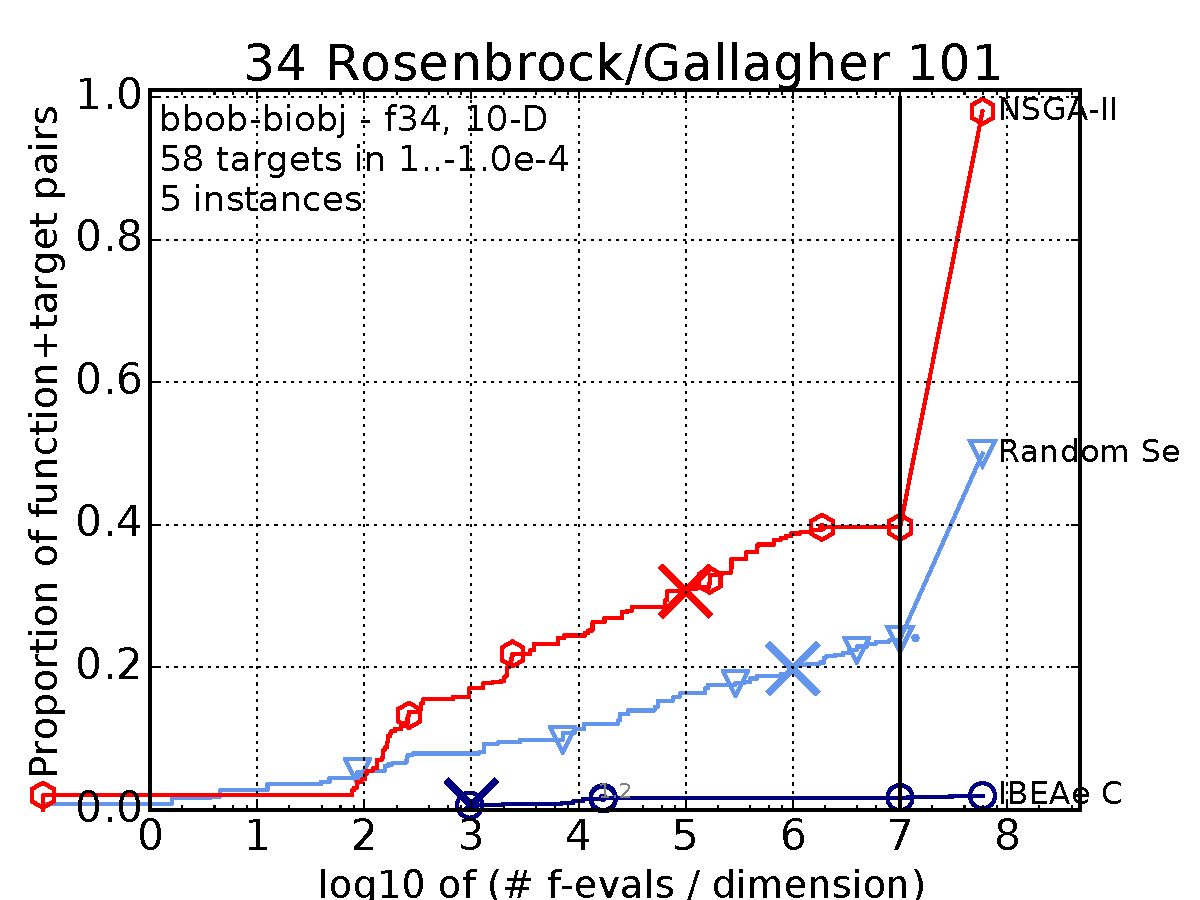
\includegraphics[width=0.2\textwidth]{pprldmany-single-functions/pprldmany_f034_10D}&
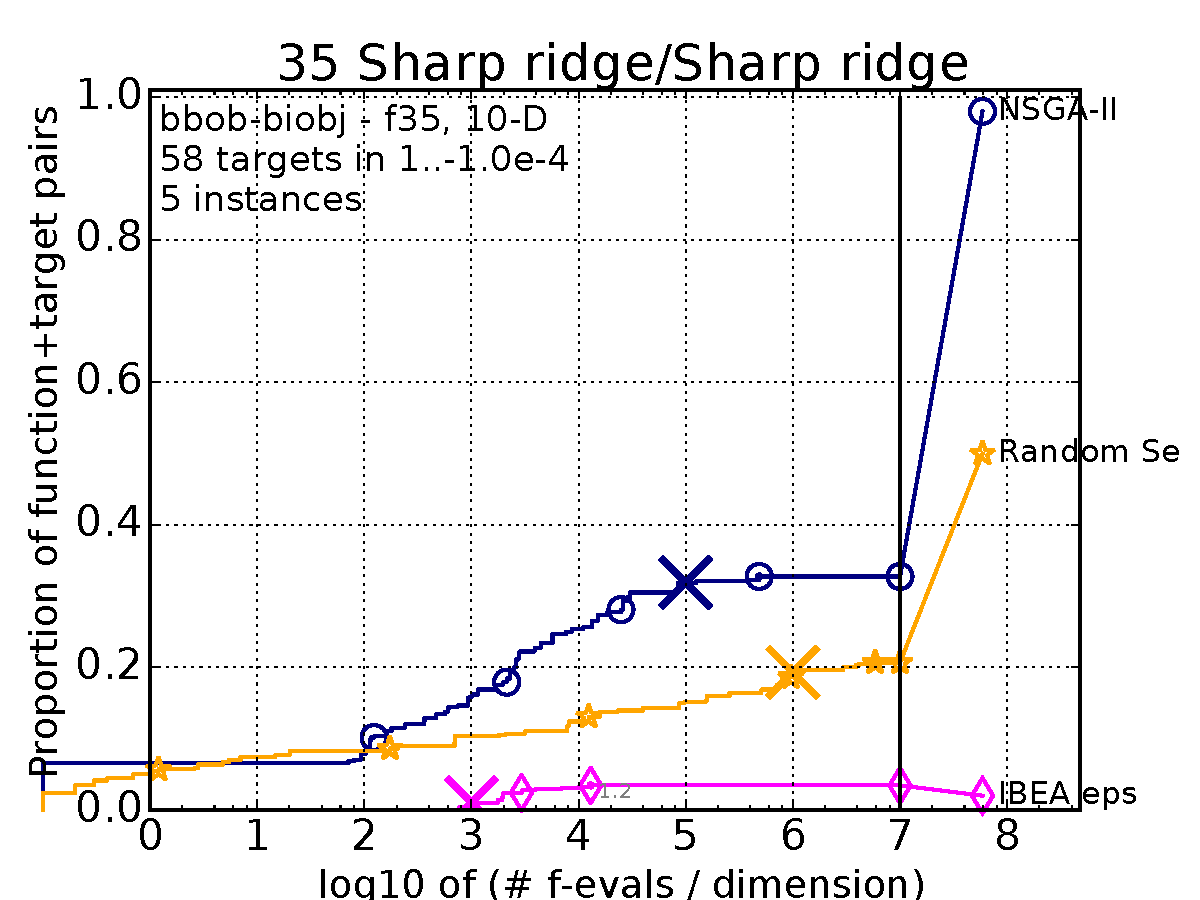
\includegraphics[width=0.2\textwidth]{pprldmany-single-functions/pprldmany_f035_10D}\\[-1.8ex]
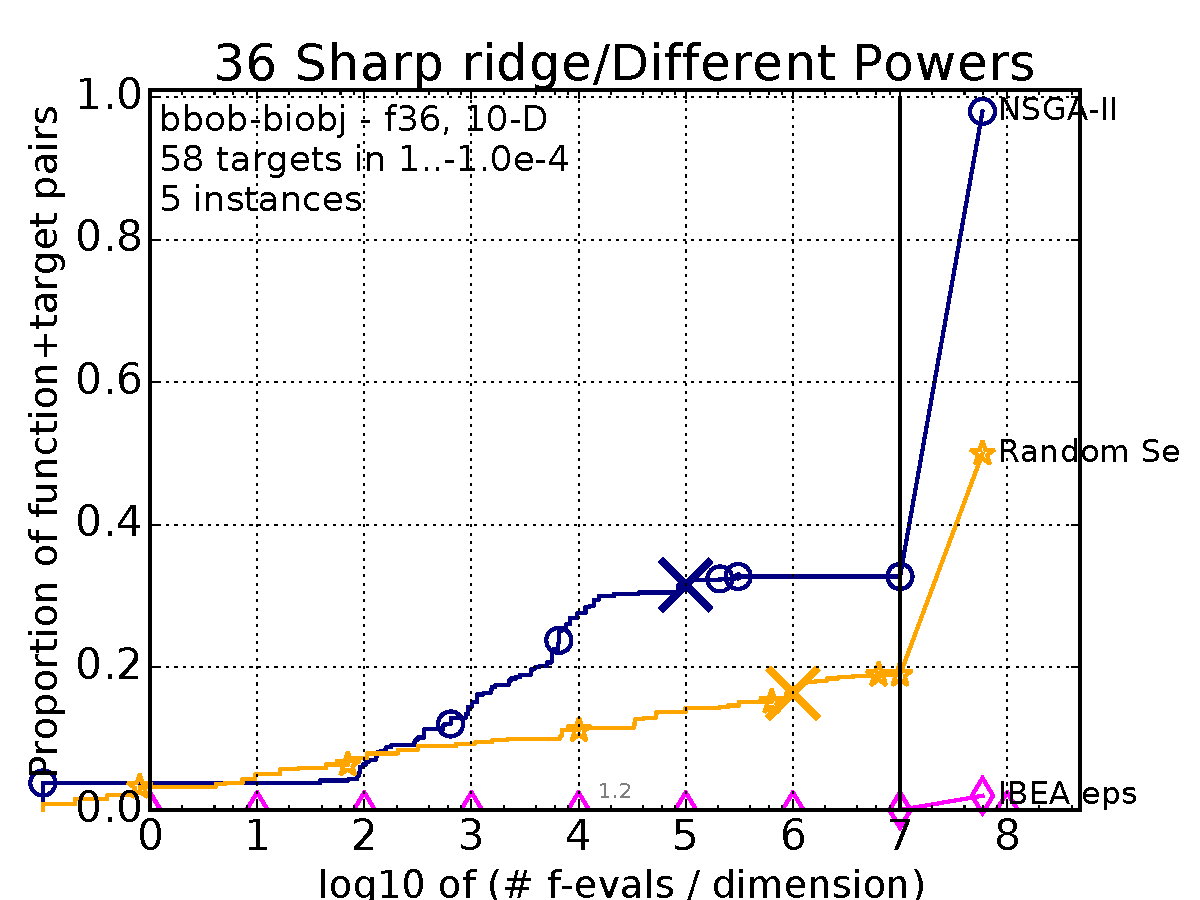
\includegraphics[width=0.2\textwidth]{pprldmany-single-functions/pprldmany_f036_10D}&
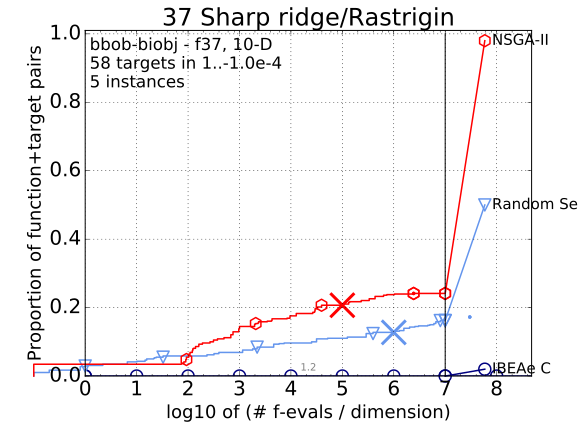
\includegraphics[width=0.2\textwidth]{pprldmany-single-functions/pprldmany_f037_10D}&
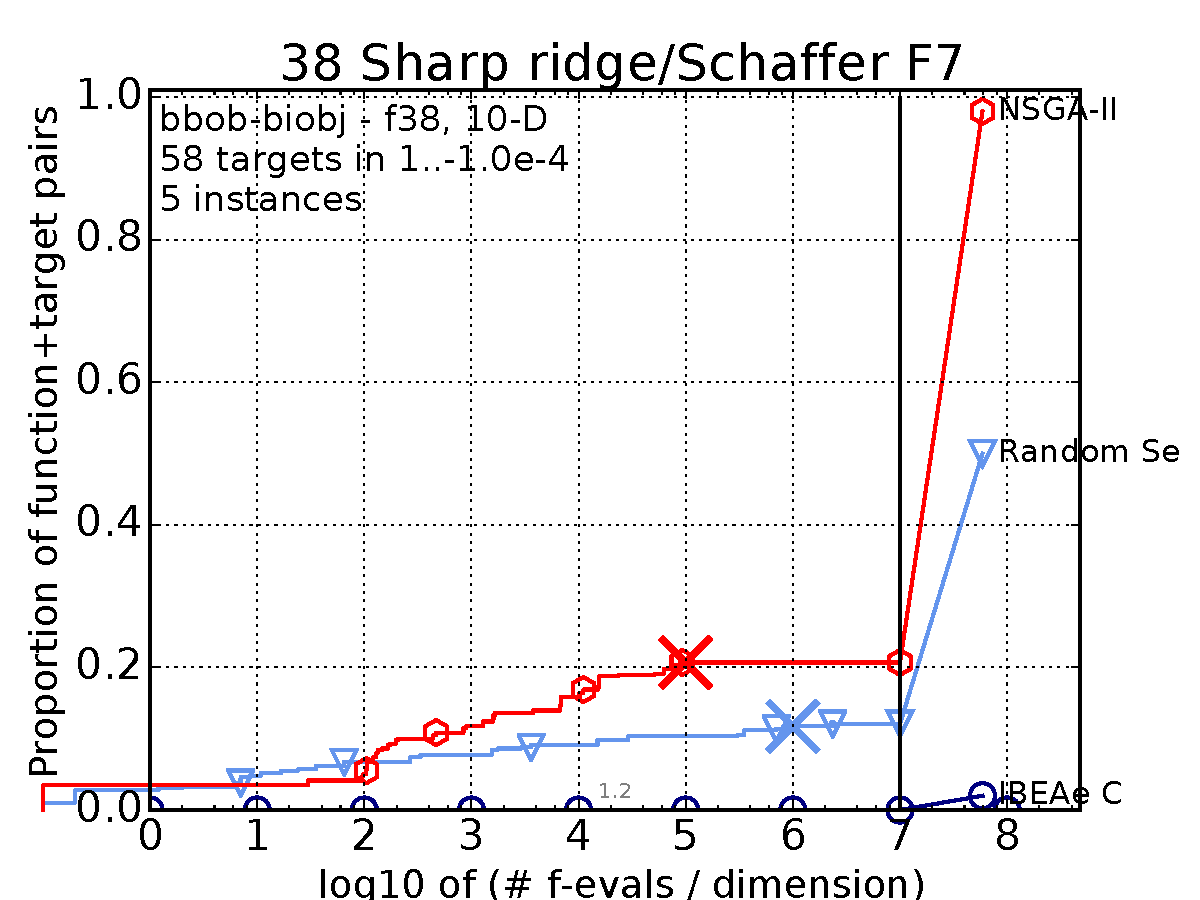
\includegraphics[width=0.2\textwidth]{pprldmany-single-functions/pprldmany_f038_10D}&
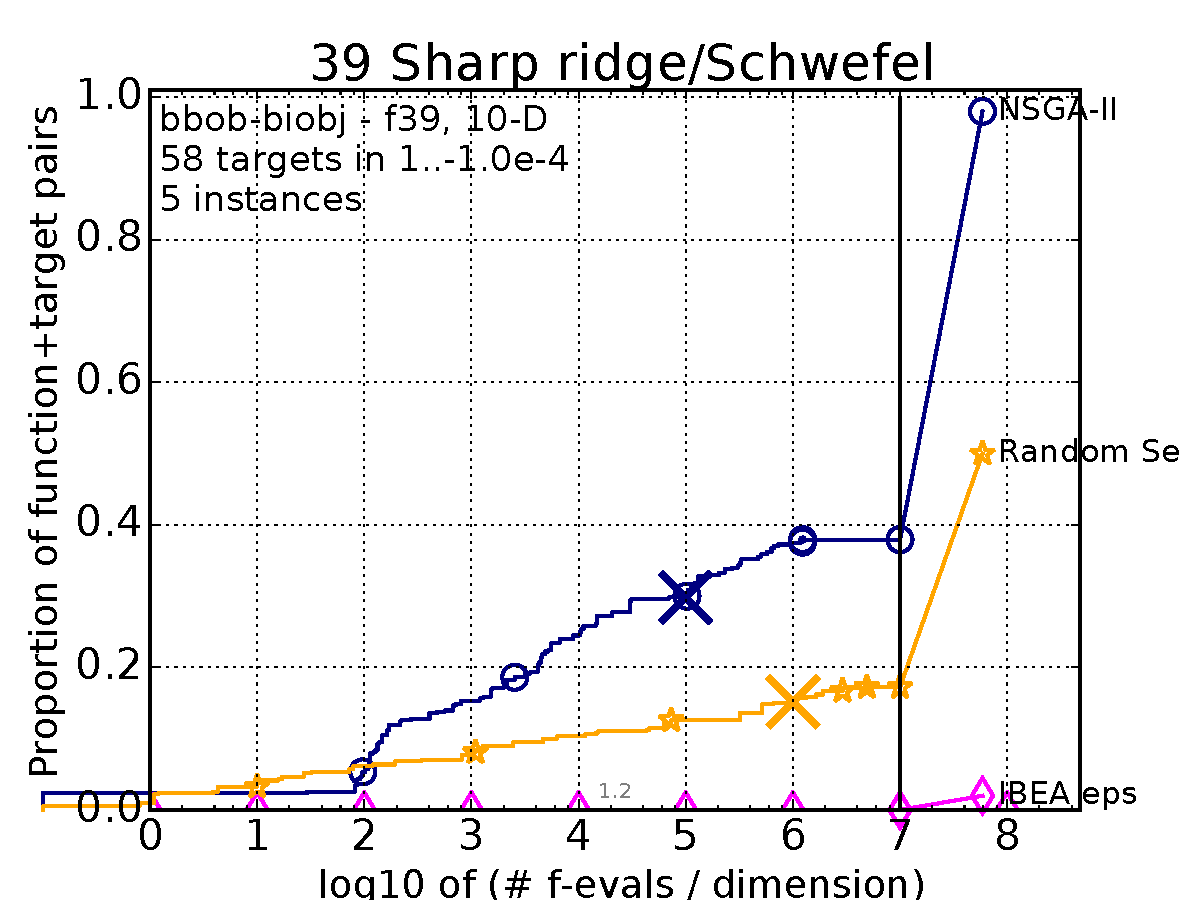
\includegraphics[width=0.2\textwidth]{pprldmany-single-functions/pprldmany_f039_10D}&
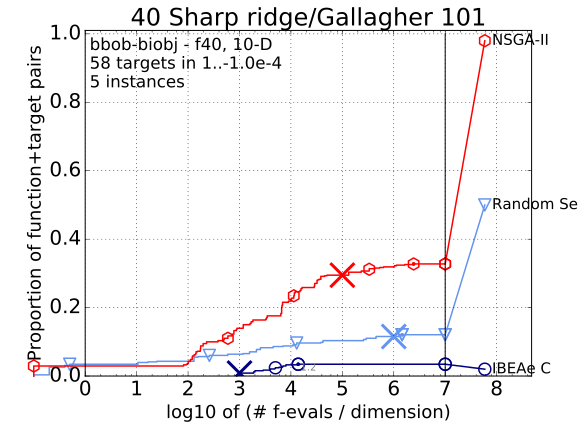
\includegraphics[width=0.2\textwidth]{pprldmany-single-functions/pprldmany_f040_10D}\\[-1.8ex]

\end{tabular}
 \caption{\label{fig:ECDFsingleOne}
 Bootstrapped empirical cumulative distribution of the number of objective function evaluations divided by dimension (FEvals/DIM) for $58$ targets with target precision in $\{-10^{-4}, -10^{-4.2}, $ $-10^{-4.4}, -10^{-4.6}, -10^{-4.8}, -10^{-5}, 0, 10^{-5}, 10^{-4.9}, 10^{-4.8}, \dots, 10^{-0.1}, 10^0\}$ for each single function $f_{1}$ to $f_{40}$ in 10-D. 
}
\end{figure*}

\begin{figure*}
\centering
\begin{tabular}{@{\hspace*{-0.005\textwidth}}l@{\hspace*{-0.005\textwidth}}l@{\hspace*{-0.005\textwidth}}l@{\hspace*{-0.005\textwidth}}l@{\hspace*{-0.005\textwidth}}l@{\hspace*{-0.005\textwidth}}}
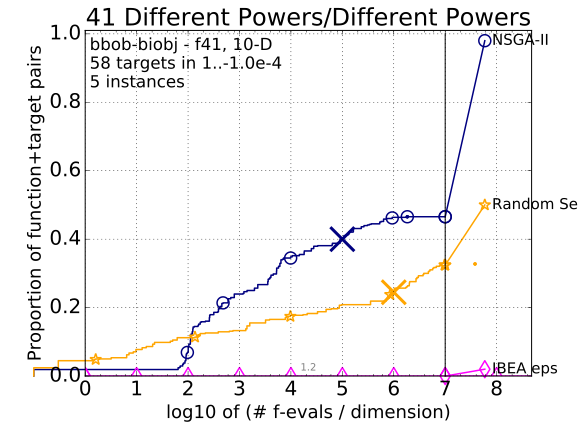
\includegraphics[width=0.2\textwidth]{pprldmany-single-functions/pprldmany_f041_10D}&
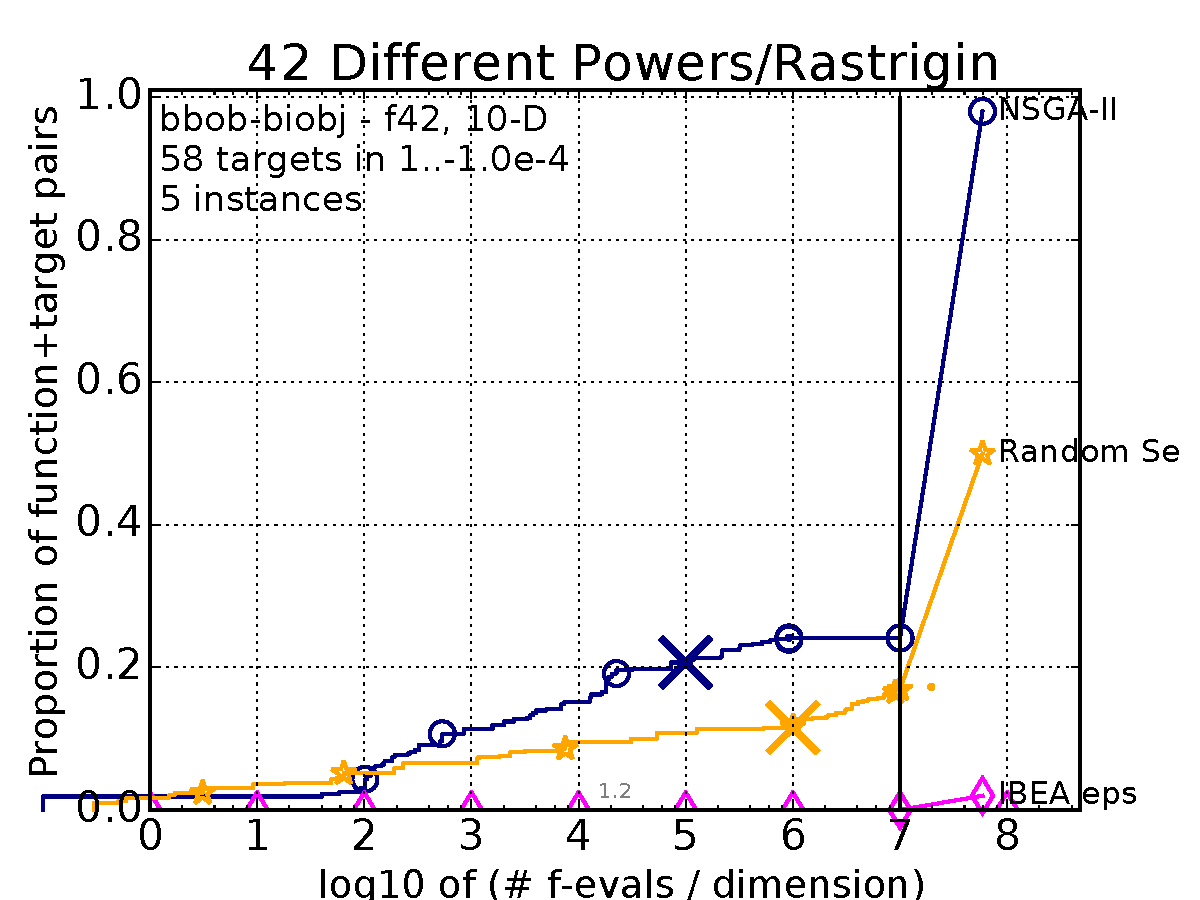
\includegraphics[width=0.2\textwidth]{pprldmany-single-functions/pprldmany_f042_10D}&
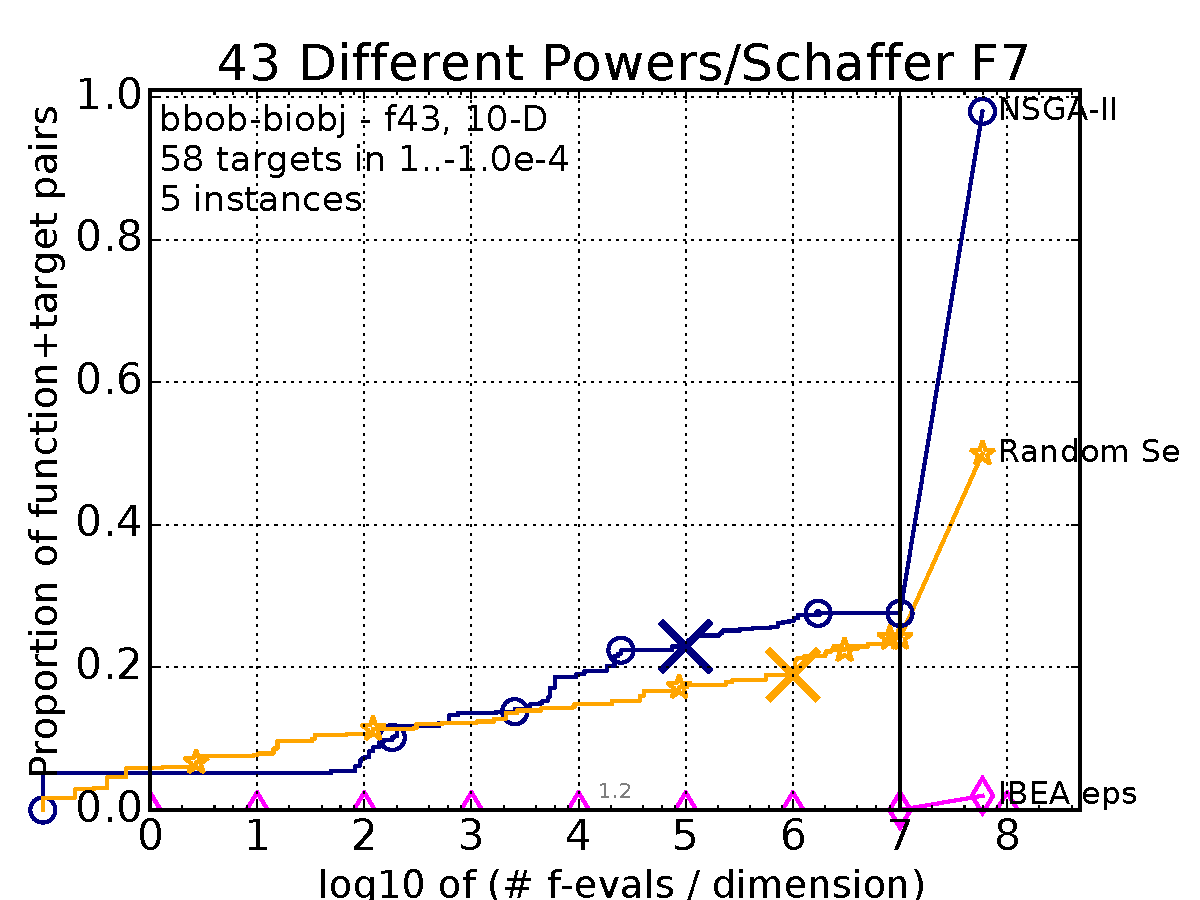
\includegraphics[width=0.2\textwidth]{pprldmany-single-functions/pprldmany_f043_10D}&
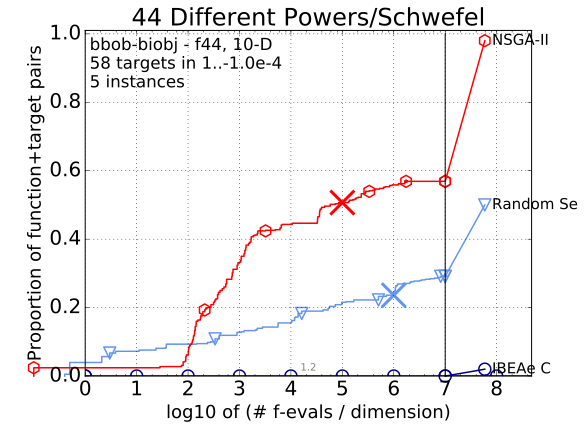
\includegraphics[width=0.2\textwidth]{pprldmany-single-functions/pprldmany_f044_10D}&
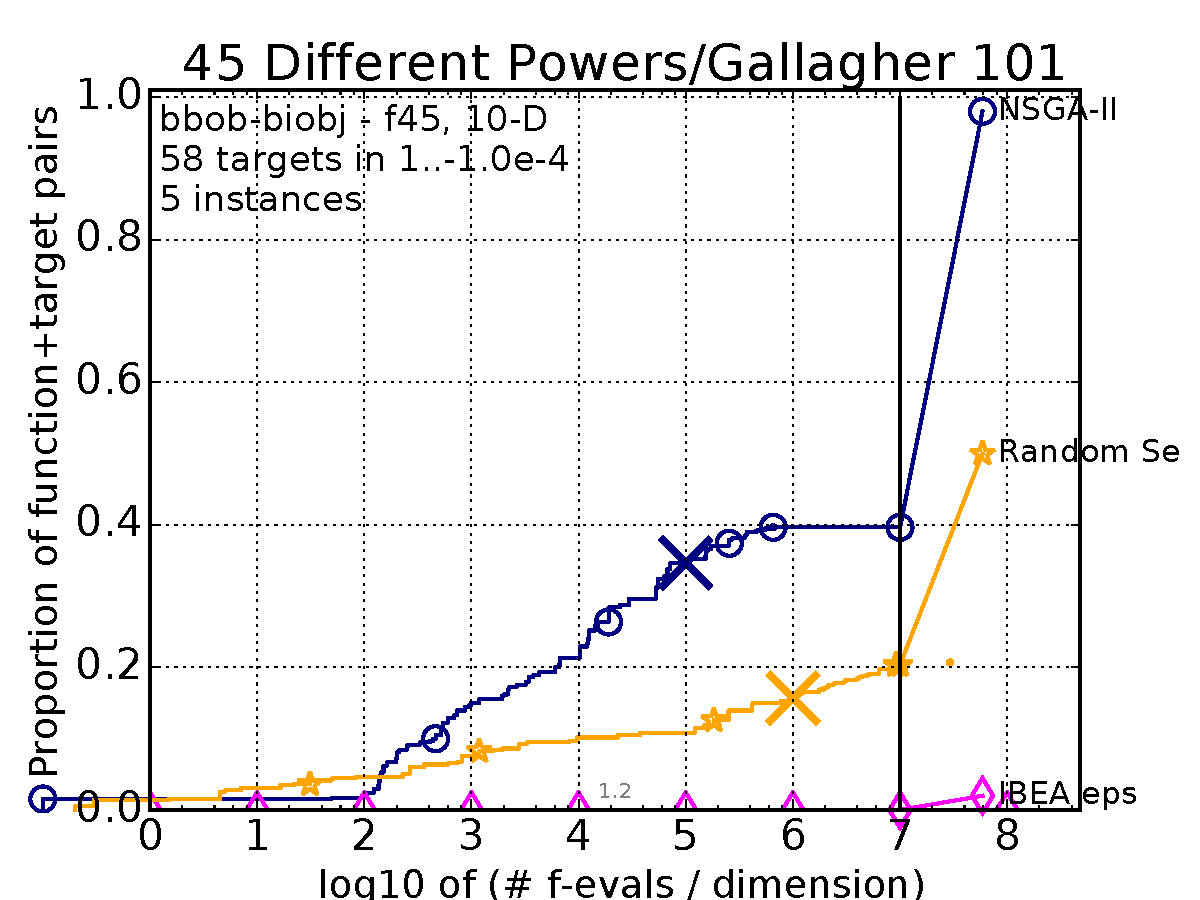
\includegraphics[width=0.2\textwidth]{pprldmany-single-functions/pprldmany_f045_10D}\\[-1.8ex]
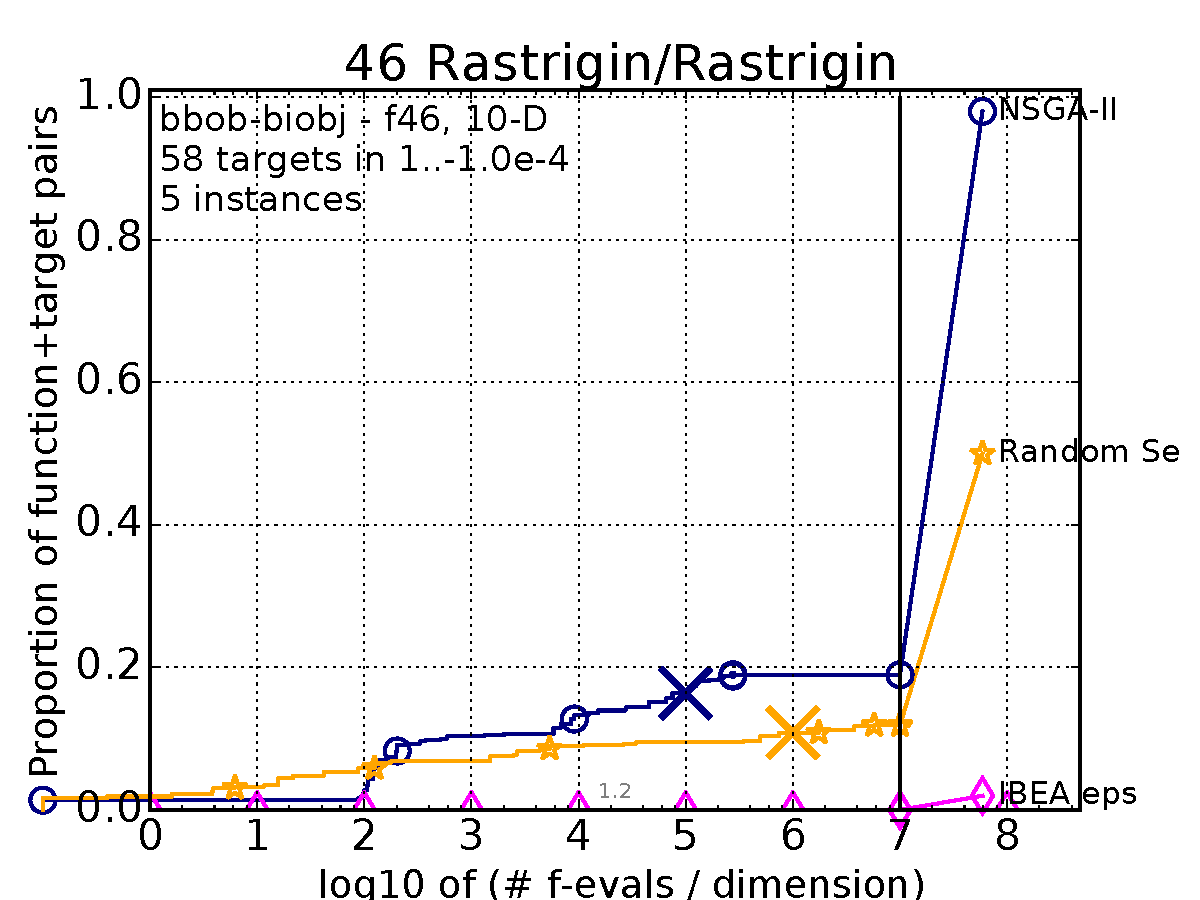
\includegraphics[width=0.2\textwidth]{pprldmany-single-functions/pprldmany_f046_10D}&
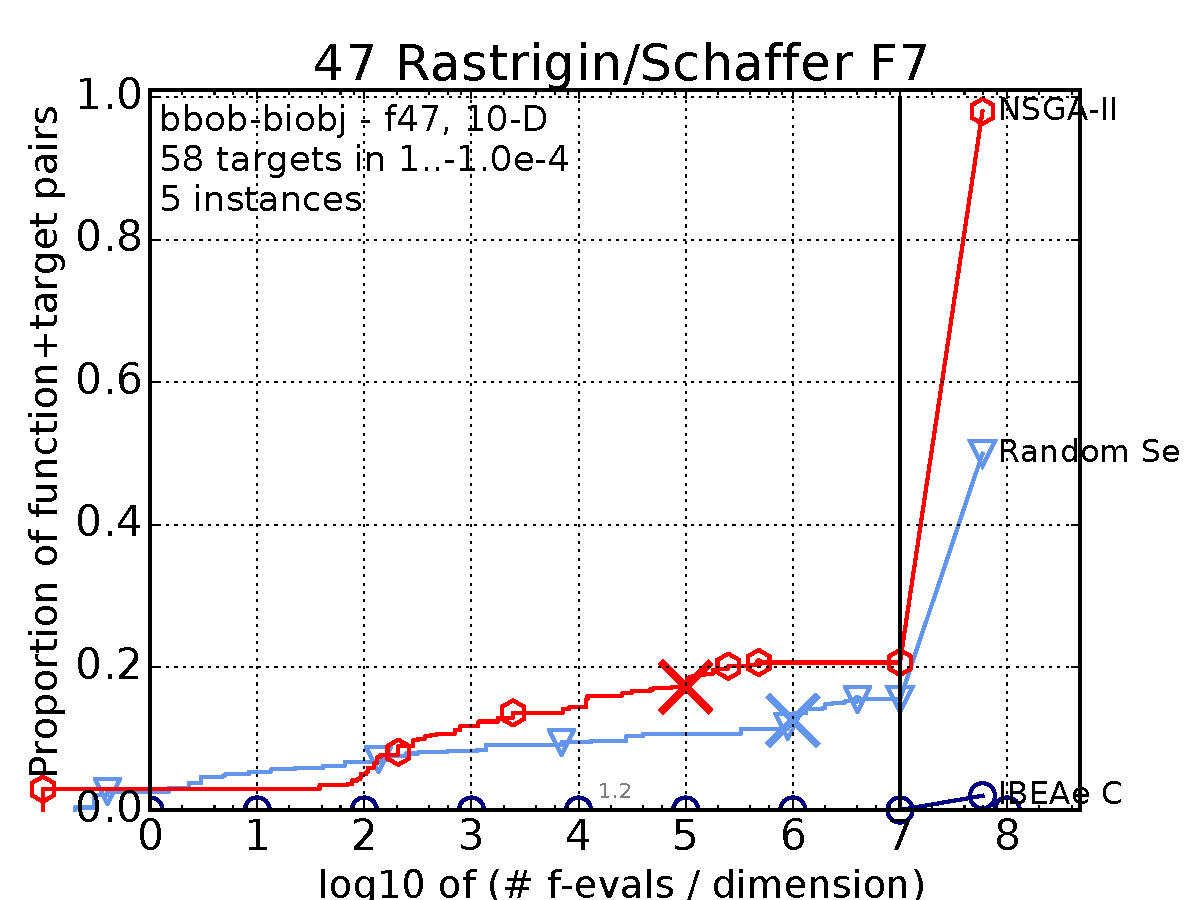
\includegraphics[width=0.2\textwidth]{pprldmany-single-functions/pprldmany_f047_10D}&
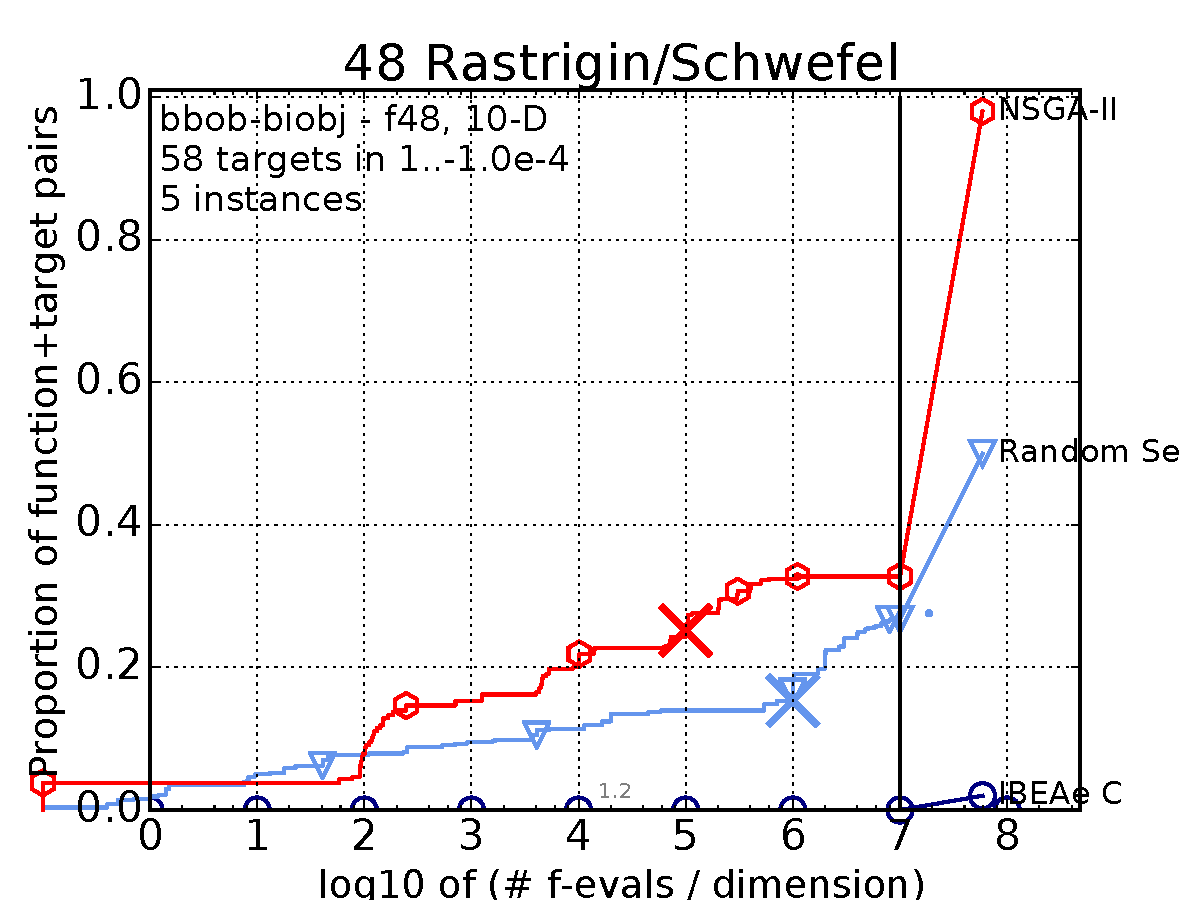
\includegraphics[width=0.2\textwidth]{pprldmany-single-functions/pprldmany_f048_10D}&
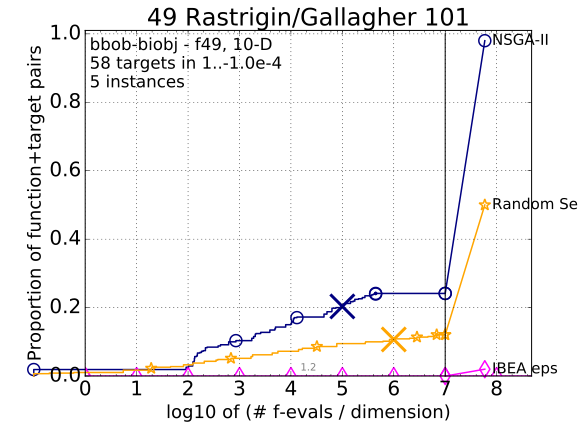
\includegraphics[width=0.2\textwidth]{pprldmany-single-functions/pprldmany_f049_10D}&
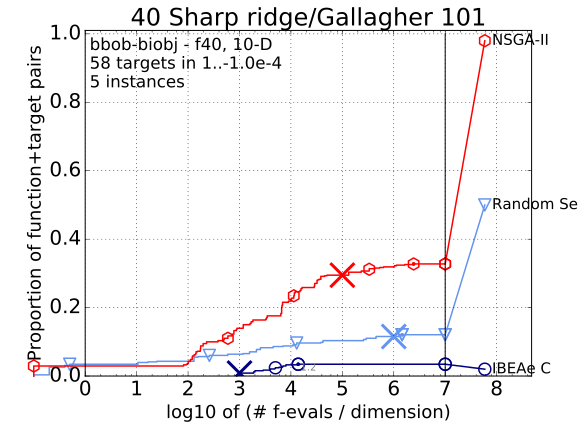
\includegraphics[width=0.2\textwidth]{pprldmany-single-functions/pprldmany_f040_10D}\\[-1.8ex]
\includegraphics[width=0.2\textwidth]{pprldmany-single-functions/pprldmany_f051_10D}&
\includegraphics[width=0.2\textwidth]{pprldmany-single-functions/pprldmany_f052_10D}&
\includegraphics[width=0.2\textwidth]{pprldmany-single-functions/pprldmany_f053_10D}&
\includegraphics[width=0.2\textwidth]{pprldmany-single-functions/pprldmany_f054_10D}&
\includegraphics[width=0.2\textwidth]{pprldmany-single-functions/pprldmany_f055_10D}\\[-1.8ex]
\end{tabular}
 \caption{\label{fig:ECDFsingleTwo}
 Bootstrapped empirical cumulative distribution of the number of objective function evaluations divided by dimension (FEvals/DIM) as in Fig.~\ref{fig:ECDFsingleOne} but for functions $f_{41}$ to $f_{55}$ in 10-D.
}
\end{figure*}




%%%%%%%%%%%%%%%%%%%%%%%%%%%%%%%%%%%%%%%%%%%%%%%%%%%%%%%%%%%%%%%%%%%%%%%%%%%%%%%
%%%%%%%%%%%%%%%%%%%%%%%%%%%%%%%%%%%%%%%%%%%%%%%%%%%%%%%%%%%%%%%%%%%%%%%%%%%%%%%

% Empirical cumulative distribution functions (ECDFs) per function group (5-D)

%%%%%%%%%%%%%%%%%%%%%%%%%%%%%%%%%%%%%%%%%%%%%%%%%%%%%%%%%%%%%%%%%%%%%%%%%%%%%%%

\begin{figure*}
\begin{tabular}{@{\hspace*{-0.009\textwidth}}c@{\hspace*{-0.014\textwidth}}c@{\hspace*{-0.016\textwidth}}c@{\hspace*{-0.02\textwidth}}c}
separable-separable & separable-moderate & separable-ill-cond. & separable-multimodal\\
\includegraphics[width=0.268\textwidth,trim=0 0 0 13mm, clip]{pprldmany_05D_1-separable_1-separable} &
\includegraphics[width=0.268\textwidth,trim=0 0 0 13mm, clip]{pprldmany_05D_1-separable_2-moderate} &
\includegraphics[width=0.268\textwidth,trim=0 0 0 13mm, clip]{pprldmany_05D_1-separable_3-ill-conditioned} &
\includegraphics[width=0.268\textwidth,trim=0 0 0 13mm, clip]{pprldmany_05D_1-separable_4-multi-modal}\\
separable-weakstructure & moderate-moderate & moderate-ill-cond. & moderate-multimodal\\
\includegraphics[width=0.268\textwidth,trim=0 0 0 13mm, clip]{pprldmany_05D_1-separable_5-weakly-structured} &
\includegraphics[width=0.268\textwidth,trim=0 0 0 13mm, clip]{pprldmany_05D_2-moderate_2-moderate} &
\includegraphics[width=0.268\textwidth,trim=0 0 0 13mm, clip]{pprldmany_05D_2-moderate_3-ill-conditioned} &
\includegraphics[width=0.268\textwidth,trim=0 0 0 13mm, clip]{pprldmany_05D_2-moderate_4-multi-modal}\\
moderate-weakstructure & ill-cond.-ill-cond. & ill-cond.-multimodal & ill-cond.-weakstructure\\
\includegraphics[width=0.268\textwidth,trim=0 0 0 13mm, clip]{pprldmany_05D_2-moderate_5-weakly-structured} &
\includegraphics[width=0.268\textwidth,trim=0 0 0 13mm, clip]{pprldmany_05D_3-ill-conditioned_3-ill-conditioned} &
\includegraphics[width=0.268\textwidth,trim=0 0 0 13mm, clip]{pprldmany_05D_3-ill-conditioned_4-multi-modal} &
\includegraphics[width=0.268\textwidth,trim=0 0 0 13mm, clip]{pprldmany_05D_3-ill-conditioned_5-weakly-structured} \\
multimodal-multimodal & multimodal-weakstructure & weakstructure-weakstructure & all 55 functions\\
\includegraphics[width=0.268\textwidth,trim=0 0 0 13mm, clip]{pprldmany_05D_4-multi-modal_4-multi-modal} &
\includegraphics[width=0.268\textwidth,trim=0 0 0 13mm, clip]{pprldmany_05D_4-multi-modal_5-weakly-structured} &
\includegraphics[width=0.268\textwidth,trim=0 0 0 13mm, clip]{pprldmany_05D_5-weakly-structured_5-weakly-structured} &
\includegraphics[width=0.268\textwidth,trim=0 0 0 13mm, clip]{pprldmany_05D_noiselessall}
\vspace*{-0.5ex}
\end{tabular}
 \caption{\label{fig:ECDFsGroupsFive}
 \bbobECDFslegend{5}
 }
\end{figure*}

%%%%%%%%%%%%%%%%%%%%%%%%%%%%%%%%%%%%%%%%%%%%%%%%%%%%%%%%%%%%%%%%%%%%%%%%%%%%%%%
%%%%%%%%%%%%%%%%%%%%%%%%%%%%%%%%%%%%%%%%%%%%%%%%%%%%%%%%%%%%%%%%%%%%%%%%%%%%%%%

% Empirical cumulative distribution functions (ECDFs) per function group (20-D)

%%%%%%%%%%%%%%%%%%%%%%%%%%%%%%%%%%%%%%%%%%%%%%%%%%%%%%%%%%%%%%%%%%%%%%%%%%%%%%%

\begin{figure*}
\begin{tabular}{@{\hspace*{-0.009\textwidth}}c@{\hspace*{-0.014\textwidth}}c@{\hspace*{-0.016\textwidth}}c@{\hspace*{-0.02\textwidth}}c}
separable-separable & separable-moderate & separable-ill-cond. & separable-multimodal\\
\includegraphics[width=0.268\textwidth,trim=0 0 0 13mm, clip]{pprldmany_20D_1-separable_1-separable} &
\includegraphics[width=0.268\textwidth,trim=0 0 0 13mm, clip]{pprldmany_20D_1-separable_2-moderate} &
\includegraphics[width=0.268\textwidth,trim=0 0 0 13mm, clip]{pprldmany_20D_1-separable_3-ill-conditioned} &
\includegraphics[width=0.268\textwidth,trim=0 0 0 13mm, clip]{pprldmany_20D_1-separable_4-multi-modal}\\
separable-weakstructure & moderate-moderate & moderate-ill-cond. & moderate-multimodal\\
\includegraphics[width=0.268\textwidth,trim=0 0 0 13mm, clip]{pprldmany_20D_1-separable_5-weakly-structured} &
\includegraphics[width=0.268\textwidth,trim=0 0 0 13mm, clip]{pprldmany_20D_2-moderate_2-moderate} &
\includegraphics[width=0.268\textwidth,trim=0 0 0 13mm, clip]{pprldmany_20D_2-moderate_3-ill-conditioned} &
\includegraphics[width=0.268\textwidth,trim=0 0 0 13mm, clip]{pprldmany_20D_2-moderate_4-multi-modal}\\
moderate-weakstructure & ill-cond.-ill-cond. & ill-cond.-multimodal & ill-cond.-weakstructure\\
\includegraphics[width=0.268\textwidth,trim=0 0 0 13mm, clip]{pprldmany_20D_2-moderate_5-weakly-structured} &
\includegraphics[width=0.268\textwidth,trim=0 0 0 13mm, clip]{pprldmany_20D_3-ill-conditioned_3-ill-conditioned} &
\includegraphics[width=0.268\textwidth,trim=0 0 0 13mm, clip]{pprldmany_20D_3-ill-conditioned_4-multi-modal} &
\includegraphics[width=0.268\textwidth,trim=0 0 0 13mm, clip]{pprldmany_20D_3-ill-conditioned_5-weakly-structured} \\
multimodal-multimodal & multimodal-weakstructure & weakstructure-weakstructure & all 55 functions\\
\includegraphics[width=0.268\textwidth,trim=0 0 0 13mm, clip]{pprldmany_20D_4-multi-modal_4-multi-modal} &
\includegraphics[width=0.268\textwidth,trim=0 0 0 13mm, clip]{pprldmany_20D_4-multi-modal_5-weakly-structured} &
\includegraphics[width=0.268\textwidth,trim=0 0 0 13mm, clip]{pprldmany_20D_5-weakly-structured_5-weakly-structured} &
\includegraphics[width=0.268\textwidth,trim=0 0 0 13mm, clip]{pprldmany_20D_noiselessall}
\vspace*{-0.5ex}
\end{tabular}
 \caption{\label{fig:ECDFsGroupsTwenty}
 \bbobECDFslegend{20}
 }
\end{figure*}


\clearpage

%%%%%%%%%%%%%%%%%%%%%%%%%%%%%%%%%%%%%%%%%%%%%%%%%%%%%%%%%%%%%%%%%%%%%%%%%%%%%%%
%%%%%%%%%%%%%%%%%%%%%%%%%%%%%%%%%%%%%%%%%%%%%%%%%%%%%%%%%%%%%%%%%%%%%%%%%%%%%%%

% Average runtime (aRT in number of function evaluations)
% for functions $f_1$--$f_{55}$ of the bbob-biobj suite for dimension 5.

%%%%%%%%%%%%%%%%%%%%%%%%%%%%%%%%%%%%%%%%%%%%%%%%%%%%%%%%%%%%%%%%%%%%%%%%%%%%%%%
\begin{table*}\tiny
\centering
\mbox{\begin{minipage}[t]{0.32\textwidth}\tiny
\centering
\input{\bbobdatapath pptables_f001_05D} 

\input{\bbobdatapath pptables_f002_05D}

\input{\bbobdatapath pptables_f003_05D}

\input{\bbobdatapath pptables_f004_05D}

\input{\bbobdatapath pptables_f005_05D}

\input{\bbobdatapath pptables_f006_05D}

\input{\bbobdatapath pptables_f007_05D}

\input{\bbobdatapath pptables_f008_05D}

\input{\bbobdatapath pptables_f009_05D}

\input{\bbobdatapath pptables_f010_05D}

\input{\bbobdatapath pptables_f011_05D}

\input{\bbobdatapath pptables_f012_05D}

\input{\bbobdatapath pptables_f013_05D}

\input{\bbobdatapath pptables_f014_05D}

\input{\bbobdatapath pptables_f015_05D}

\input{\bbobdatapath pptables_f016_05D}

\input{\bbobdatapath pptables_f017_05D}

\input{\bbobdatapath pptables_f018_05D}

\input{\bbobdatapath pptables_f019_05D}

\end{minipage}
\hspace{0.002\textwidth}
\begin{minipage}[t]{0.32\textwidth}\tiny
\centering

\input{\bbobdatapath pptables_f020_05D}

\input{\bbobdatapath pptables_f021_05D}

\input{\bbobdatapath pptables_f022_05D}

\input{\bbobdatapath pptables_f023_05D}

\input{\bbobdatapath pptables_f024_05D}

\input{\bbobdatapath pptables_f025_05D}

\input{\bbobdatapath pptables_f026_05D}

\input{\bbobdatapath pptables_f027_05D}

\input{\bbobdatapath pptables_f028_05D}

\input{\bbobdatapath pptables_f029_05D}

\input{\bbobdatapath pptables_f030_05D}

\input{\bbobdatapath pptables_f031_05D}

\input{\bbobdatapath pptables_f032_05D}

\input{\bbobdatapath pptables_f033_05D}

\input{\bbobdatapath pptables_f034_05D}

\input{\bbobdatapath pptables_f035_05D}

\input{\bbobdatapath pptables_f036_05D}

\input{\bbobdatapath pptables_f037_05D}

\end{minipage}

\hspace{0.002\textwidth}
\begin{minipage}[t]{0.32\textwidth}\tiny
\centering

\input{\bbobdatapath pptables_f038_05D}

\input{\bbobdatapath pptables_f039_05D}

\input{\bbobdatapath pptables_f040_05D}

\input{\bbobdatapath pptables_f041_05D}

\input{\bbobdatapath pptables_f042_05D}

\input{\bbobdatapath pptables_f043_05D}

\input{\bbobdatapath pptables_f044_05D}

\input{\bbobdatapath pptables_f045_05D}

\input{\bbobdatapath pptables_f046_05D}

\input{\bbobdatapath pptables_f047_05D}

\input{\bbobdatapath pptables_f048_05D}

\input{\bbobdatapath pptables_f049_05D}

\input{\bbobdatapath pptables_f050_05D}

\input{\bbobdatapath pptables_f051_05D}

\input{\bbobdatapath pptables_f052_05D}

\input{\bbobdatapath pptables_f053_05D}

\input{\bbobdatapath pptables_f054_05D}

\input{\bbobdatapath pptables_f055_05D}

\end{minipage}}

 \caption{\label{tab:aRTs5}
 \bbobpptablesmanylegend{dimension $5$}{110} % Bonferroni correction: #dimensions * #functions
 }
\end{table*}
%sideways


%%%%%%%%%%%%%%%%%%%%%%%%%%%%%%%%%%%%%%%%%%%%%%%%%%%%%%%%%%%%%%%%%%%%%%%%%%%%%%%
%%%%%%%%%%%%%%%%%%%%%%%%%%%%%%%%%%%%%%%%%%%%%%%%%%%%%%%%%%%%%%%%%%%%%%%%%%%%%%%

% Average runtime (aRT in number of function evaluations)
% for functions $f_1$--$f_{55}$ of the bbob-biobj suite for dimension 20.

%%%%%%%%%%%%%%%%%%%%%%%%%%%%%%%%%%%%%%%%%%%%%%%%%%%%%%%%%%%%%%%%%%%%%%%%%%%%%%%
\begin{table*}\tiny
\centering
\mbox{\begin{minipage}[t]{0.32\textwidth}\tiny
\centering
\input{\bbobdatapath pptables_f001_20D} 

\input{\bbobdatapath pptables_f002_20D}

\input{\bbobdatapath pptables_f003_20D}

\input{\bbobdatapath pptables_f004_20D}

\input{\bbobdatapath pptables_f005_20D}

\input{\bbobdatapath pptables_f006_20D}

\input{\bbobdatapath pptables_f007_20D}

\input{\bbobdatapath pptables_f008_20D}

\input{\bbobdatapath pptables_f009_20D}

\input{\bbobdatapath pptables_f010_20D}

\input{\bbobdatapath pptables_f011_20D}

\input{\bbobdatapath pptables_f012_20D}

\input{\bbobdatapath pptables_f013_20D}

\input{\bbobdatapath pptables_f014_20D}

\input{\bbobdatapath pptables_f015_20D}

\input{\bbobdatapath pptables_f016_20D}

\input{\bbobdatapath pptables_f017_20D}

\input{\bbobdatapath pptables_f018_20D}

\input{\bbobdatapath pptables_f019_20D}

\end{minipage}
\hspace{0.002\textwidth}
\begin{minipage}[t]{0.32\textwidth}\tiny
\centering

\input{\bbobdatapath pptables_f020_20D}

\input{\bbobdatapath pptables_f021_20D}

\input{\bbobdatapath pptables_f022_20D}

\input{\bbobdatapath pptables_f023_20D}

\input{\bbobdatapath pptables_f024_20D}

\input{\bbobdatapath pptables_f025_20D}

\input{\bbobdatapath pptables_f026_20D}

\input{\bbobdatapath pptables_f027_20D}

\input{\bbobdatapath pptables_f028_20D}

\input{\bbobdatapath pptables_f029_20D}

\input{\bbobdatapath pptables_f030_20D}

\input{\bbobdatapath pptables_f031_20D}

\input{\bbobdatapath pptables_f032_20D}

\input{\bbobdatapath pptables_f033_20D}

\input{\bbobdatapath pptables_f034_20D}

\input{\bbobdatapath pptables_f035_20D}

\input{\bbobdatapath pptables_f036_20D}

\input{\bbobdatapath pptables_f037_20D}

\end{minipage}

\hspace{0.002\textwidth}
\begin{minipage}[t]{0.32\textwidth}\tiny
\centering

\input{\bbobdatapath pptables_f038_20D}

\input{\bbobdatapath pptables_f039_20D}

\input{\bbobdatapath pptables_f040_20D}

\input{\bbobdatapath pptables_f041_20D}

\input{\bbobdatapath pptables_f042_20D}

\input{\bbobdatapath pptables_f043_20D}

\input{\bbobdatapath pptables_f044_20D}

\input{\bbobdatapath pptables_f045_20D}

\input{\bbobdatapath pptables_f046_20D}

\input{\bbobdatapath pptables_f047_20D}

\input{\bbobdatapath pptables_f048_20D}

\input{\bbobdatapath pptables_f049_20D}

\input{\bbobdatapath pptables_f050_20D}

\input{\bbobdatapath pptables_f051_20D}

\input{\bbobdatapath pptables_f052_20D}

\input{\bbobdatapath pptables_f053_20D}

\input{\bbobdatapath pptables_f054_20D}

\input{\bbobdatapath pptables_f055_20D}

\end{minipage}}

 \caption{\label{tab:aRTs20}
 \bbobpptablesmanylegend{dimension $20$}{110} % Bonferroni correction: #dimensions * #functions
 }
\end{table*}



%%%%%%%%%%%%%%%%%%%%%%%%%%%%%%%%%%%%%%%%%%%%%%%%%%%%%%%%%%%%%%%%%%%%%%%%%%%%%%%
%%%%%%%%%%%%%%%%%%%%%%%%%%%%%%%%%%%%%%%%%%%%%%%%%%%%%%%%%%%%%%%%%%%%%%%%%%%%%%%
%
% The following two commands are all you need in the
% initial runs of your .tex file to
% produce the bibliography for the citations in your paper.
\bibliographystyle{abbrv}
\bibliography{bbob}  % bbob.bib is the name of the Bibliography in this case
% You must have a proper ".bib" file
%  and remember to run:
% latex bibtex latex latex
% to resolve all references
% to create the ~.bbl file.  Insert that ~.bbl file into
% the .tex source file and comment out
% the command \texttt{{\char'134}thebibliography}.
%
% ACM needs 'a single self-contained file'!
%

% \clearpage % otherwise the last figure might be missing
\end{document}
